% Chapter Template

\chapter{Ensayos y resultados} % Main chapter title
\label{Chapter4}
En este capítulo se presentan los resultados de los estudios realizados sobre los modelos de predicción de PLC y CHF. 

\section{Estimación de PLC}
A continuación, se presentan los resultados para el modelo de estimación de PLC: la optimización de hiperparámetros, las predicciones de DNBR y fracción de vacío del mejor modelo y la estimación de PLC por ambos criterios.

\subsection{Optimización de hiperparámetros}
Como se mencionó en la sección \ref{sec:plc_arq}, la optimización de hiperparámetros se realizó por medio de la biblioteca Optuna. Las métricas objetivo se establecieron por separado para cada criterio. Para el DNBR se utilizó el error porcentual medio, mientras que para la fracción de vacío se usó el error absoluto medio escalado 100 veces. Esta decisión se tomó al considerar que la fracción de vacío tiene valor exactamente igual a 0 para un porcentaje importante de los datos y con el objetivo de lograr una contribución equitativa de ambos criterios al rendimiento del modelo. De esta forma, se obtiene un único modelo con error similar en ambos criterios y se evita entrenar uno por cada uno de ellos.

La figura \ref{fig:plc_opt_results} muestra los resultados durante el proceso de optimización, mientras que la arquitectura final se resume en la tabla \ref{tab:plc_arq_hp}.

\begin{table}[H]
	\centering
	\caption{Hiperparámetros de la arquitectura final.}
	\begin{tabular}{l c}    
        \toprule
        \textbf{Hiperparámetro} & \textbf{Valor} \\
        \hline
        Cantidad de capas ocultas & $3$ \\
        Cantidad de neuronas por capa & $478$ \\
        Learning rate & $1.38 \cdot 10^{-4}$ \\
        Batch & 64 \\
        Función de activación & ReLU \\
		\bottomrule
	\end{tabular}
	\label{tab:plc_arq_hp}
\end{table}

\begin{figure}[H]
    \centering
    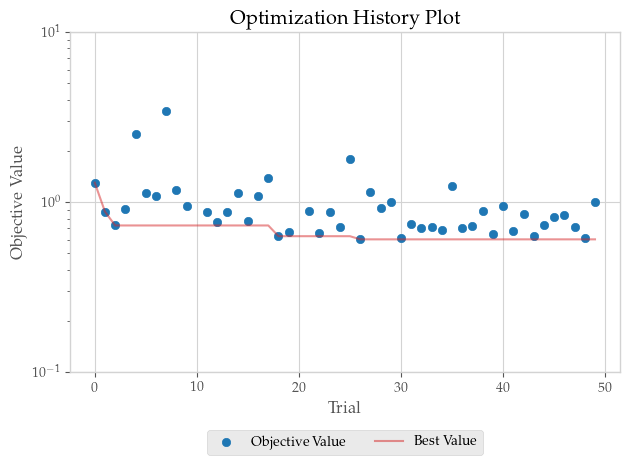
\includegraphics[width=0.7\textwidth]{Figures/plc_opt_result.png}
    \caption{Resultados de los distintos intentos de la optimización.}
    \label{fig:plc_opt_results}
\end{figure}

\subsection{Resultados de DNBR y fracción de vacío}

En esta sección, se evalúan los resultados del modelo en cuanto a la predicción de DNBR y fracción de vacío. En la figura \ref{fig:plc_results_dnbr_vacio} se presentan los gráficos de valores predichos contra reales, para los conjuntos de test y train. Se observa una buena predicción del modelo en ambos objetivos y una distribución equivalente entre conjuntos. No obstante, se aprecia una tendencia a subestimar la fracción de vacío en la región cercana a 25\%.

\begin{figure}[h]
    \centering
    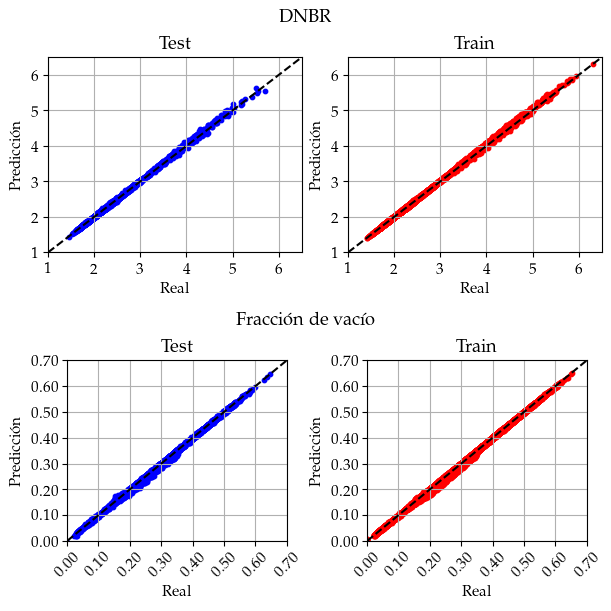
\includegraphics[width=0.8\textwidth]{Figures/plc_pred.png}
    \caption{Resultados de predicción de DNBR y fracción de vacío, para los conjuntos de test y train.}
    \label{fig:plc_results_dnbr_vacio}
\end{figure}

En la tabla \ref{tab:plc_errors_dnbr_vacio} se presentan la media y el desvío estándar del error con signo para cada objetivo. El error con signo se define como la diferencia entre el valor real y el predicho, por lo que valores positivos de la media implican una subpredicción del objetivo, y los negativos una sobrepredicción. Para la fracción de vacío, se aplica un factor de 10 para que las magnitudes entre objetivos sean comparables. Se observa una tendencia a subpredecir DNBR y a sobrepredecir la fracción de vacío, ambas tendencias en igual magnitud en train y test. Los desvíos estándar son menores en test que en train para DNBR, y a la inversa para la fracción de vacío. En ambos casos, los valores de desvío estándar son bajos. 

La tendencia general de la predicción de vacío es a sobrepredecir, mientras que el gráfico de predicho contra real indica lo contrario. Para analizar esta discrepancia, se realizó el mismo cálculo del error al dividir en 5 regiones el dominio de cada variable objetivo. Los resultados se presentan en la tabla \ref{tab:plc_errors_dnbr_vacio_segmentado}. Se obtiene, para DNBR, una media aún más baja en la región de interés ($1.7-2.5$) y una subpredicción general del DNBR, lo que representa una tendencia conservativa. En cuanto a la fracción de vacío, no se tiene el mínimo de error en la zona de interés, sino alrededor de ella. En la zona de interés ($0.15-0.35$) se tiene una sobrepredicción de la fracción de vacío, también una tendencia conservativa. Se puede concluir entonces que el modelo tiene un buen rendimiento en ambos objetivos y tendencias conservativas respecto de las referencias.

\begin{table}[h]
	\centering
	\caption{Media y desvío estándar del error con signo para cada objetivo.}
	\begin{tabular}{c c c c c} 
        \toprule
        \multirow{2}{*}{\textbf{Conjunto}} & \multicolumn{2}{c}{\textbf{DNBR}} & \multicolumn{2}{c}{\textbf{Fracción de vacío}} \\
                & media     & $\sigma$  & media & $\sigma$  \\
        Train   & $-0.006$    & $0.021$     & $0.018$ & $0.040$     \\
        Test    & $-0.006$    & $0.017$     & $0.018$ & $0.032$     \\
		\bottomrule
	\end{tabular}
	\label{tab:plc_errors_dnbr_vacio}
\end{table}

\begin{table}[h]
	\centering
	\caption{Media y desvío estándar del error con signo para cada objetivo, segmentado por rangos de cada objetivo.}
	\begin{tabular}{c c c c c c} 
        \toprule
        \multirow{3}{1.5cm}{\textbf{Objetivo}} & \multirow{3}{*}{\textbf{Rango}} & \multicolumn{4}{c}{\textbf{Conjunto}} \\
        &                                               & \multicolumn{2}{c}{Train} & \multicolumn{2}{c}{Test} \\ 
        &                                               & media & $\sigma$  & media & $\sigma$  \\
        \multirow{5}{1.5cm}{DNBR}               
                        &$   <1.7$  & $0.003$ &   $0.004$   & $0.000$ &  $0.008$    \\ 
                        &$1.7-2.5$  & $-0.001$&   $0.009$   & $-0.001$&  $0.013$    \\
                        &$2.5-3.5$  & $-0.013$&   $0.013$   & $-0.015$&  $0.019$    \\
                        &$  3.5-5$  & $-0.044$&   $0.038$   & $-0.042$&  $0.051$    \\
                        &$     >5$  & $-0.051$&   $0.039$   & $-0.015$&  $0.076$    \\
        \hline
        \multirow{5}{1.5cm}{Fracción de vacío}
                        &$        0$  & $-0.035$ & $0.033$ & $0.061$ & $0.037$ \\ 
                        &$   0-0.15$  &  $0.013$ & $0.021$ & $0.010$ & $0.032$ \\
                        &$0.15-0.35$  &  $0.024$ & $0.036$ & $0.025$ & $0.044$ \\
                        &$ 0.35-0.6$  &  $0.007$ & $0.021$ & $0.007$ & $0.027$ \\
                        &$     >0.6$  &  $0.031$ & $0.022$ & $0.024$ & $0.014$ \\

		\bottomrule
	\end{tabular}
	\label{tab:plc_errors_dnbr_vacio_segmentado}
\end{table}

Como se explicó en la sección \ref{sec:plc_pipeline}, se filtraron los datos disponibles para entrenar en la región de interés en ambas variables objetivo. El filtro conservó los valores de MDNBR entre $1.7$ y $2.5$, o de fracción de vacío entre 15\% y 35\%. Por ello, resulta de interés evaluar la precisión del modelo por fuera de la región de entrenamiento. En la figura \ref{fig:plc_results_excluidos} se presentan las predicciones comparadas con los valores reales, para MDNBR y fracción de vacío.
En primer lugar, se evidencia la dificultad del modelo para predecir en las regiones excluidas del entrenamiento, algo esperable en una arquitectura DNN.
Luego, para DNBR se observa un comportamiento correcto en valores inferiores a los de interés, pero una tendencia a subpredecir al aumentar. Si bien esto podría interpretarse generalmente como un resultado desfavorable, se puede considerar que el modelo entrega predicciones conservativas fuera de su zona de entrenamiento y brinda seguridad en su aplicación. Por último, para la fracción de vacío, por debajo de la zona de interés se observan predicciones menores a 0, lo que constituye un resultado no físico. Se podría realizar un clipping de la predicción para que los valores negativos se conviertan en 0, lo que daría un buen rendimiento por debajo de la zona de entrenamiento. Por encima de la zona de entrenamiento, se puede observar en primer lugar una tendencia a subpredecir hasta 60\% y luego una sobrepredicción. 

Para cuantificar el aumento del error en el conjunto excluido, la figura \ref{fig:plc_errores} presenta los errores para cada variable objetivo en los conjuntos de train, test y excluidos. Tal como se comentó previamente, los conjuntos de train y test presentan errores muy similares, y el conjunto excluido un error considerablemente mayor. Adicionalmente, se grafican los cuantiles del 5\% y 95\%, que evidencian que el conjunto de excluidos también tiene una dispersión mucho mayor en su error.

\begin{figure}[H]
    \centering
    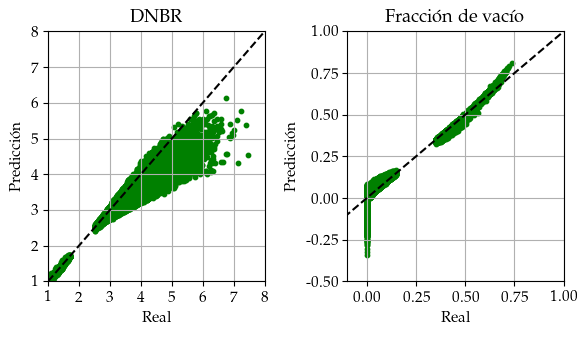
\includegraphics[width=0.8\textwidth]{Figures/plc_pred_excluidos.png}
    \caption{Resultados de predicción de DNBR y fracción de vacío, para el conjunto excluido.}
    \label{fig:plc_results_excluidos}
\end{figure}

\begin{figure}[H]
    \centering
    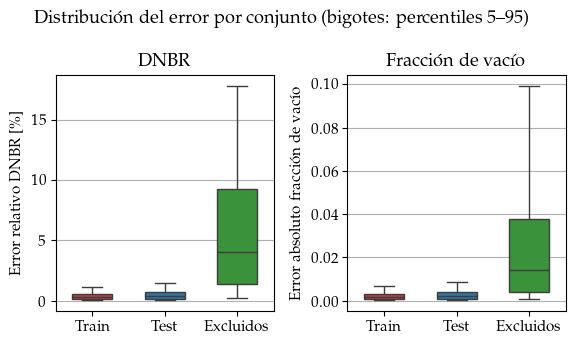
\includegraphics[width=0.8\textwidth]{Figures/plc_error.png}
    \caption{Distribución del error para cada objetivo, por conjunto de datos.}
    \label{fig:plc_errores}
\end{figure}

\subsection{Estimación de PLC por DNBR y fracción de vacío}
La evaluación del modelo realizada hasta aquí responde a su capacidad de estimar el mínimo DNBR y la fracción de vacío a la salida de un canal refrigerante, dadas sus condiciones termohidráulicas y distribuciones de potencia. Sin embargo, este no es el objetivo último del modelo, sino que se debe estimar la PLC por DNBR y fracción de vacío. Esto responde a un lazo de cálculo iterativo, explicado en detalle en la sección \ref{sec:plc_integracion}. A continuación, se analiza el comportamiento del modelo en dicho escenario, por medio del criterio del factor de ajuste $F_\mathrm{PLC}$ explicado en la sección \ref{sec:plc_evaluacion}.

Para esta evaluación, se utilizaron 100 estados del reactor correspondientes a una estrategia de recambio de elementos combustibles de la \cna{}, con un total de $43\,811$ simulaciones. El cálculo de las PLC se realizó con COBRA3-CP según la metodología tradicional, para obtener los valores de referencia y los tiempos requeridos en este tipo de cálculos. 

En la figura \ref{fig:plc_results_corr} se presentan los resultados, segmentados por ZH, para la versión base de la DNN y con la corrección por $F_\mathrm{PLC}$. En la tabla \ref{tab:plc_f} se observan los valores de media y desvío estándar para el cociente entre el valor predicho y el real, y el $F_\mathrm{PLC}$, factor de ajuste para asegurar con 95\% de probabilidad y confianza que la PLC predicha está por debajo de la real. Los tres valores se encuentran segmentados por ZH y para los criterios de DNBR y fracción de vacío.

Se observa un buen desempeño, especialmente para las ZZHH 4 y 5, donde la nube de puntos azul, correspondiente a la DNN sin corregir, se encuentra muy cerca de la recta identidad. Para las ZZHH 1 a 3, el desempeño es inferior, aunque los resultados se encuentran dentro de parámetros aceptables. Este comportamiento resulta esperable, ya que en el conjunto de datos de entrenamiento la representación de las ZZHH era equivalente a la cantidad de canales de cada una en el reactor, distribución que es muy despareja. Esto también se evidencia en los valores de media y desvío estándar del cociente predicho-real. La media y el desvío estándar son decrecientes de ZH 1 a 5, con un valor casi unitario en la última. Los factores de ajuste muestran una mayor sobreestimación de las PLC en las ZZHH periféricas.

Debe tenerse en cuenta que para las ZZHH 1 a 3 el límite siempre se obtiene por fracción de vacío. Por lo tanto, el error en predicción de DNBR no es un problema, y el buen rendimiento en fracción de vacío hace al modelo apto para predecir en estas ZZHH. La ZH 4, en este caso, también está limitada por vacío, por lo que se le puede aplicar la misma conclusión.

En la tabla \ref{tab:plc_tiempos} se presenta un resumen de los tiempos de cómputo para el cálculo de PLC. Los resultados son contundentes: la mejora o speedup del proceso de cálculo alcanza una media de entre $8\,409$ y $9\,519$ para DNBR, y de entre $2\,197$ y $2\,486$ para fracción de vacío. El tiempo total de cómputo pasó de las 380 h con COBRA3-CP a alrededor de 4 minutos con la DNN. Esto sustenta el valor de este modelo, que no solo logra una predicción de las PLC con un error acotado, sino que además requiere un tiempo de cómputo varios órdenes de magnitud inferior. Por otra parte, no se implementaron lógicas adicionales para lograr un cómputo más eficiente por medio de la DNN, como el procesamiento en batch. Se computaron todos los casos en serie, tanto en CPU como en GPU. Estos aspectos representan oportunidades de mejora, como se explica en el capítulo \ref{Chapter5}.

\begin{figure}[hbtp]
    \centering
    % 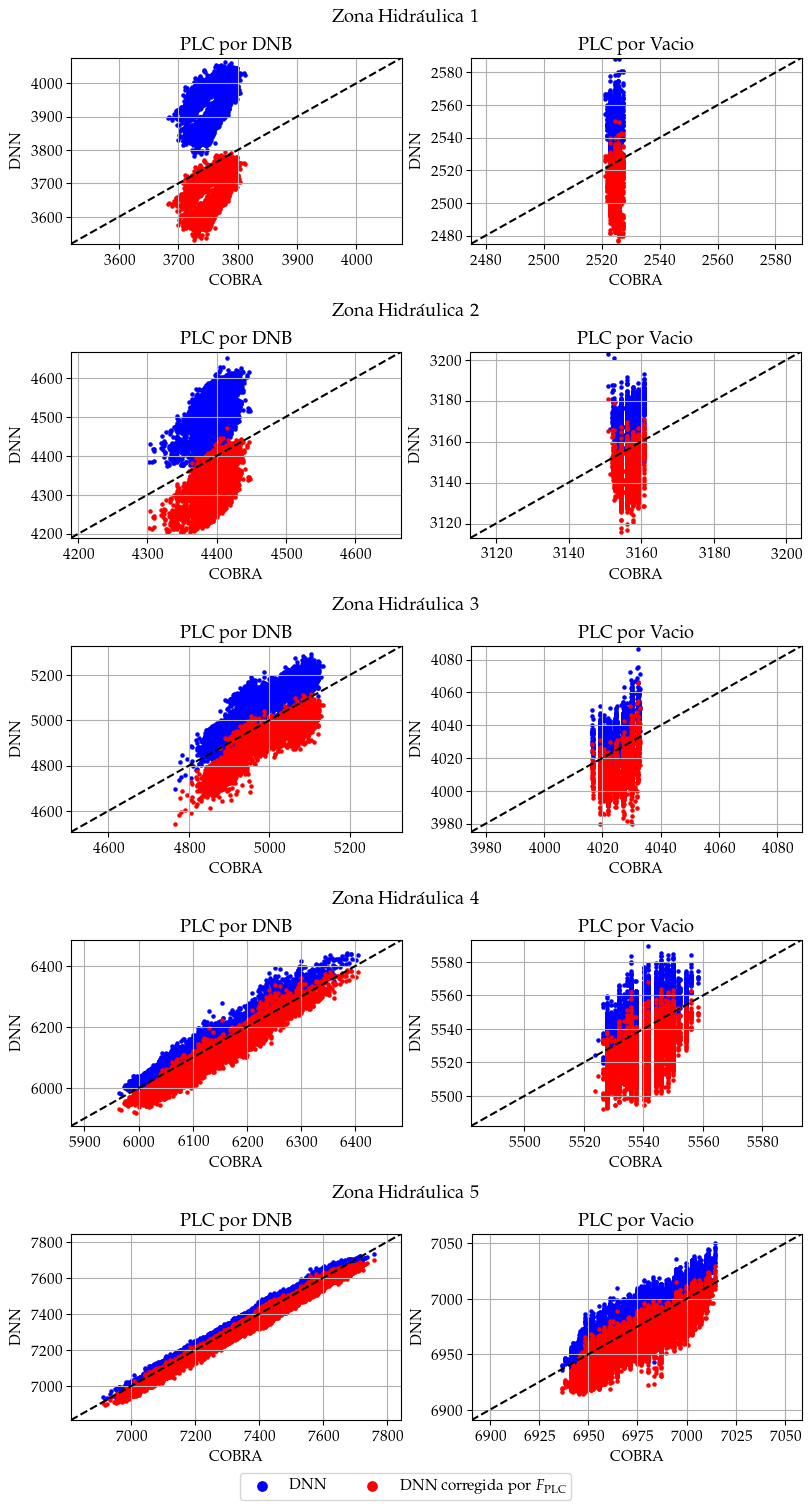
\includegraphics[width=\textwidth]{Figures/plc_pred_corr.png}
    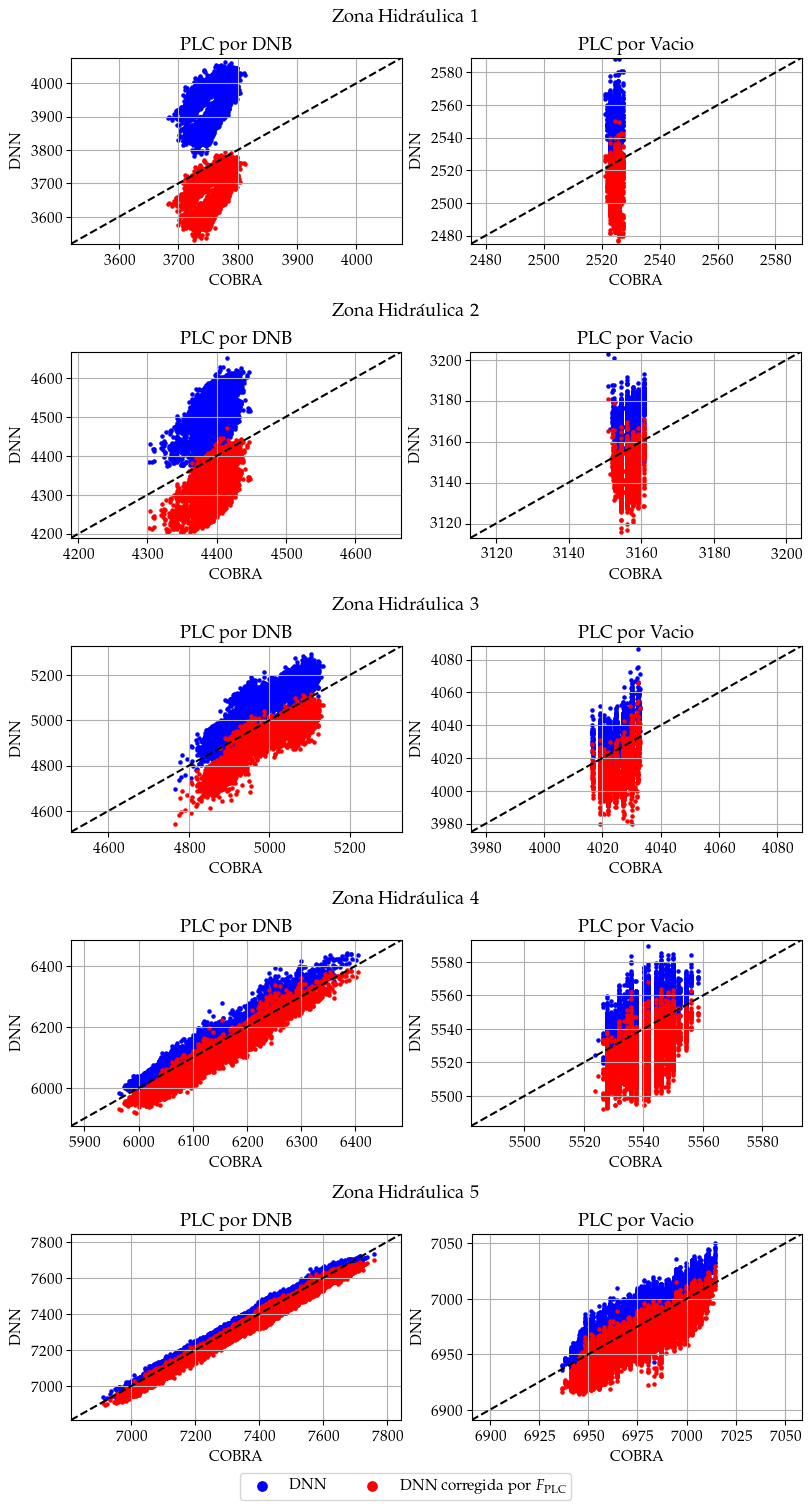
\includegraphics[height=\textheight]{Figures/plc_pred_corr.png}
    \caption{Resultados de estimación de PLC por DNBR y fracción de vacío con factor de corrección, por zona hidráulica.}
    \label{fig:plc_results_corr}
\end{figure}

\begin{table}[H]
	\centering
	\caption{Media y desvío estándar de cociente predicho-real, y factor de 95\% de probabilidad y confianza. Por zona hidráulica.}
	\begin{tabular}{c c c c c c c } 
        \toprule
        \multirow{2}{*}{\textbf{Zona Hidráulica}} & \multicolumn{3}{c}{\textbf{DNBR}} & \multicolumn{3}{c}{\textbf{Fracción de vacío}} \\
            & media & $\sigma$  & F     & media & $\sigma$  & F     \\
        1 & $1.047$ & $0.015$ & $0.933$ & $1.008$ & $0.004$ & $0.985$ \\
        2 & $1.025$ & $0.010$ & $0.961$ & $1.003$ & $0.002$ & $0.993$ \\
        3 & $1.018$ & $0.010$ & $0.967$ & $1.002$ & $0.002$ & $0.995$ \\
        4 & $1.003$ & $0.003$ & $0.991$ & $1.001$ & $0.002$ & $0.996$ \\
        5 & $1.001$ & $0.002$ & $0.995$ & $1.001$ & $0.001$ & $0.997$ \\
		\bottomrule
	\end{tabular}
	\label{tab:plc_f}
\end{table}

\begin{table}[H]
	\centering
	\caption{Tiempos de cómputo para cálculo de PLC.}
	\begin{tabular}{l l c c c c c} 
        \toprule
        & & \multicolumn{3}{c}{\textbf{Tiempo}} & \multicolumn{2}{c}{\multirow{2}{*}{\textbf{Mejora}}} \\
        & & \multirow{2}{*}{\textbf{COBRA3-CP [s]}} & \multicolumn{2}{c}{\textbf{DNN [ms]}} &  \\
        & &                                     & CPU & GPU & CPU & GPU \\
        \hline
        \multirow{4}{1.5cm}{DNBR}   
                                & mínimo        & $8.53$      & $0.28$  & $0.47$ & 3 562   & 406 \\
                                & media         & $25.16$     & $2.66$  & $3.03$ & 9 519   & 8 409\\
                                & máximo        & $137.95$    & $5.88$  & $5.51$ & 57 882 & 48 363\\
                                & \textbf{total}& 306 h     & 117 s & 130 s& 9 445  & 8 503\\
        \hline
        \multirow{4}{1.5cm}{Fracción de vacío}  
                                & mínimo        & $1.07$      & $0.21$  & $0.33$  & 432   & 405\\
                                & media         & $6.09$      & $2.46$  & $2.80$  & 2 486  & 2 197\\
                                & máximo        & $14.70$     & $5.70$  & $6.69$  & 5 955  & 5 385\\
                                & \textbf{total}& 74 h     & 108 s & 120 s & 2 479  & 2 224\\
		\bottomrule
	\end{tabular}
	\label{tab:plc_tiempos}
\end{table}

Por último, en la tabla \ref{tab:plc_margen_perdido} se observan los márgenes de potencia perdidos al aplicar la predicción de DNN. Es decir, la diferencia porcentual de potencia entre el valor de referencia y el predicho, corregido por $F_\mathrm{PLC}$. Se presentan los valores de margen medio y de margen máximo. Luego se computa el total como el promedio ponderado por la cantidad de canales que pertenecen a cada ZH.
Se obtuvieron valores decrecientes de la ZH 1 a la 5 tanto por DNBR como por fracción de vacío, a excepción de la ZH 3, que presenta el valor máximo de margen perdido por DNBR. Los valores máximos en las zonas periféricas resultan altos, aunque dentro de los porcentajes de margen tomados como criterio de seguridad al calcular una estrategia de recambio de combustibles.
Es importante tener en cuenta que las ZZHH 1 a 4 están actualmente limitadas por fracción de vacío, y la ZH 5 por DNBR. 

Finalmente, los márgenes perdidos totales medios son del $0.7$\% para DNBR y $0.5$\% para fracción de vacío. Esto expresa la capacidad del modelo de predecir con precisión y seguridad la PLC, sin un resultado demasiado conservativo. Además, debe tenerse en cuenta que las zonas periféricas operan con un importante margen, muy superior al perdido por la utilización del modelo para fracción de vacío. Por lo tanto, el margen expuesto como perdido en rigor no se pierde.

\begin{table}[H]
	\centering
	\caption{Margen perdido medio y máximo por utilizar DNN, según zona hidráulica y total.}
	\begin{tabular}{c c c c c } 
        \toprule
        \multirow{3}{*}{\textbf{Zona Hidráulica}} & \multicolumn{4}{c}{\textbf{Margen perdido [\%]}} \\ \cline{2-5}
        & \multicolumn{2}{c}{\textbf{DNBR}} & \multicolumn{2}{c}{\textbf{Fracción de vacío}} \\
          & medio & máximo & medio & máximo \\ \hline
        1 & $1.56$ & $4.56$ & $2.58$ & $5.22$ \\
        2 & $1.35$ & $4.29$ & $1.05$ & $2.28$ \\
        3 & $1.88$ & $5.37$ & $0.74$ & $1.87$ \\
        4 & $0.58$ & $2.12$ & $0.41$ & $1.25$ \\
        5 & $0.38$ & $1.37$ & $0.24$ & $0.89$ \\ \hline
        \textbf{total} & $0.71$ & $2.34$ & $0.54$ & $1.45$ \\
		\bottomrule
	\end{tabular}
	\label{tab:plc_margen_perdido}
\end{table}

\subsection{Aplicación de embeddings}
Como se explicó en la sección \ref{sec:arq_embeddings}, se aplicó una arquitectura de autoencoder para obtener el espacio latente de los perfiles de potencia axial y por barras. La arquitectura empleada fue simple, ya que esta tarea no requiere una red densa. Se optó por un encoder con 2 capas ocultas, la primera de 64 neuronas y la segunda de 32. El decoder, por su parte, es el espejo del encoder.

Se buscó el espacio latente de menor dimensión tal que la reconstrucción del vector de entrada en el conjunto de entrenamiento tuviera un coeficiente de determinación $\mathrm{R}^2>0.99$. El proceso de cálculo recorrió desde un espacio latente de dimensión 1 hasta la primera dimensión que cumpliera con la condición establecida. Para el entrenamiento se utilizó el mismo conjunto de datos que para el estimador de PLC.

Para ambos perfiles de potencia se obtuvo un espacio latente de 3 dimensiones. En la figura \ref{fig:embeddings_axial} se presentan, para cada componente del espacio latente, los 3 perfiles con mayor valor de la componente, los 3 con valores medianos y los 3 con menor valor. La primera componente puede interpretarse como el clásico factor de forma de los perfiles axiales, donde los perfiles de menor valor corresponden a la forma típicamente llamada ``panza arriba''. La segunda componente tiene un significado similar; se asocia con perfiles cuya zona inferior o superior está aplanada. Por último, la tercera componente representa potencia disminuida en el centro del perfil.

\begin{figure}[H]
    \centering
    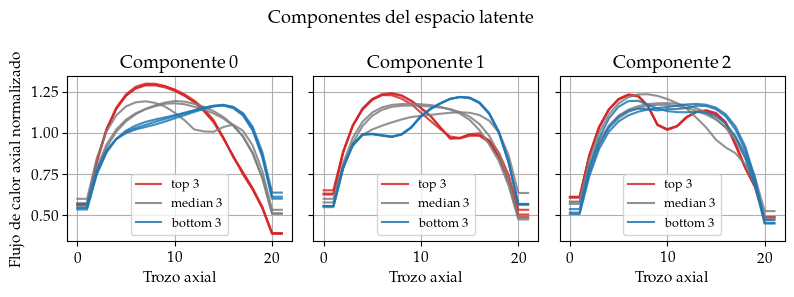
\includegraphics[width=\textwidth]{Figures/embeddings_axial_componentes_latente.png}
    \caption{Gráficos de perfiles axiales con valores más altos, medianos y bajos de cada componente del espacio latente.}
    \label{fig:embeddings_axial}
\end{figure}

En la figura \ref{fig:embeddings_radial} se presenta el gráfico análogo para el perfil por barras. En este caso, resulta más difícil obtener una explicación de cada componente.

\begin{figure}[hbtp]
    \centering
    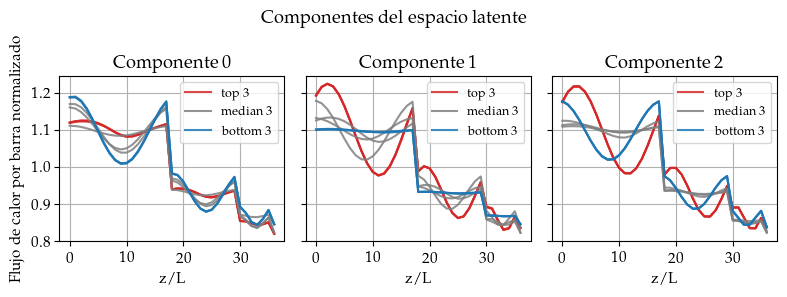
\includegraphics[width=\textwidth]{Figures/embeddings_radial_componentes_latente.png}
    \caption{Gráficos de perfiles radiales con valores más altos, medianos y bajos de cada componente del espacio latente.}
    \label{fig:embeddings_radial}
\end{figure}

Una vez entrenado el encoder, se evaluó la arquitectura del predictor de PLC, pero con el espacio latente de los perfiles de potencia como entradas. Se plantearon tres modelos, que utilizan el espacio latente del perfil axial, el del perfil por barras y ambos espacios latentes. En la tabla \ref{tab:plc_emb_errors_dnbr_vacio} se presentan la media y el desvío estándar del error con signo, para los tres modelos con embeddings y el modelo base. Los tres modelos presentan una reducción de la media del error en ambas variables objetivo. En cuanto al desvío estándar, para DNBR no se obtiene una reducción significativa, pero para fracción de vacío se reduce a aproximadamente la mitad. Es importante señalar que los modelos con embeddings del perfil por barras y de ambos perfiles presentan una media positiva del error de DNBR. Por otro lado, los tres modelos presentan un error medio negativo para la fracción de vacío. Estos dos puntos son un resultado no conservativo, aunque no de forma excesiva.

\begin{table}[h]
	\centering
	\caption{Media y desvío estándar del error con signo para cada objetivo, para modelos con embeddings.}
	\begin{tabular}{l c c c c c} 
        \toprule
        \multirow{2}{*}{\textbf{Modelo}} & \multirow{2}{*}{\textbf{Conjunto}} & \multicolumn{2}{c}{\textbf{DNBR}} & \multicolumn{2}{c}{\textbf{Fracción de vacío}} \\
        &         & media     & $\sigma$  & media & $\sigma$  \\ \hline
        \multirow{2}{*}{Base}
        & Train   &  $-0.006$    & $0.021$     & $0.018$ & $0.040$ \\
        & Test    &  $-0.006$    & $0.017$     & $0.018$ & $0.032$ \\ \hline
        \multirow{2}{*}{Emb. perfil axial}
        & Train   & $-0.002$ & $0.018$ & $-0.002$ & $0.021$ \\
        & Test    & $-0.001$ & $0.020$ & $-0.002$ & $0.022$   \\   \hline
        \multirow{2}{*}{Emb. perfil por barras}
        & Train   & $0.001$ & $0.013$ & $-0.006$ & $0.021$ \\
        & Test    & $0.001$ & $0.014$ & $-0.006$ & $0.022$ \\   \hline
        \multirow{2}{*}{Emb. ambos perfiles}
        & Train   & $0.000$ & $0.017$ & $-0.011$ & $0.016$ \\
        & Test    & $0.000$ & $0.020$ & $-0.010$ & $0.017$ \\

		\bottomrule
	\end{tabular}
	\label{tab:plc_emb_errors_dnbr_vacio}
\end{table}

En la tabla \ref{tab:plc_emb_margen_perdido} se presenta el margen perdido total para el modelo base y los tres modelos con embeddings. En cuanto al DNBR, solo el modelo con embeddings para el perfil por barras presenta una reducción del margen perdido. Para el margen perdido de fracción de vacío se obtiene una reducción en los tres modelos.

Se estima que la reducción del margen perdido en la PLC por DNBR al utilizar el espacio latente del perfil por barras proviene de la elevada dimensión de dicho perfil, en relación con la información que representa. Al reducir su dimensión, la DNN tendría mayor capacidad de centrar recursos en otras variables de entrada. 

En el caso de la PLC por fracción de vacío, es sabido que depende de la integral de la energía entregada y no de condiciones locales. Por lo tanto, variables de entrada globales como las componentes del espacio latente presentan una ventaja esperable en su predicción.

\begin{table}[H]
	\centering
	\caption{Margen perdido medio y máximo por utilizar DNN y embeddings, según zona hidráulica y total.}
	\begin{tabular}{c c c c c} 
        \toprule
        \multirow{3}{*}{\textbf{Modelo}} & \multicolumn{4}{c}{\textbf{Margen perdido [\%]}} \\ \cline{2-5}
        & \multicolumn{2}{c}{\textbf{DNBR}} & \multicolumn{2}{c}{\textbf{Fracción de vacío}} \\
          & medio & máximo & medio & máximo \\ \hline
        Base & $0.71$ & $2.34$ & $0.54$ & $1.45$ \\
        Emb. perfil axial       & $0.84$ & $3.05$ & $0.13$ & $0.39$ \\
        Emb. perfil por barras  & $0.61$ & $1.83$ & $0.15$ & $0.38$ \\
        Emb. ambos perfiles     & $0.99$ & $3.96$ & $0.10$ & $0.40$ \\
		\bottomrule
	\end{tabular}
	\label{tab:plc_emb_margen_perdido}
\end{table}

\newpage
\section{Estimación de CHF}

A continuación, se analizan los resultados para el modelo de estimación de CHF.
En primer lugar, se presenta el modelo predictor de CHF para geometría de tubo, a partir de los datos recopilados por Groeneveld \citep{GROENEVELD2007, USNRC2019NUREGKM0011}. Esto permite establecer una base sólida sobre la que los modelos de multifidelidad corrigen la estimación para un tubo de forma no lineal.

Luego, se presentan dos análisis respecto de la arquitectura del modelo. Ya que el trabajo propone una superposición de arquitecturas, se evalúa la contribución de cada cambio, con la referencia de un modelo simple y de la metodología actual. Se evalúa en primer lugar la arquitectura de multifidelidad, con la referencia de una implementación de una DNN tradicional. En segundo lugar, se evalúa la implementación de PINN a la red de multifidelidad, con la referencia de la arquitectura de multifidelidad base.

En tercer lugar, se analizan las variables de entrada al modelo, ya que su uso sin evaluación equivale a un modelo de caja negra, que no permite comprender su comportamiento ni su relación con la física del fenómeno. 
Citando a von Neumann: ``Con cuatro parámetros puedo ajustar un elefante, y con cinco puedo hacer que mueva su trompa''\footnotemark{}.
\footnotetext{Traducido de la frase original en inglés: ``With four parameters I can fit an elephant, and with five I can make him wiggle his trunk'' \citep{dyson2004meeting}.}
Tanto este análisis como los de arquitectura se realizaron con una penalización al modelo: se entrenó sobre casos de caudal alto y se evaluó sobre casos de caudal bajo.

Por último, se define el modelo final, entrenado con una división aleatoria de los datos. Se comparan los valores de \dnbrmin{} para las arquitecturas \mfdnn{} y \mfpinn{}. Luego se realiza una estimación del impacto de los valores obtenidos con un cálculo de PLC con las condiciones del diseño termohidráulico descriptas en el IFS.

\subsection{Modelo predictor de CHF en un tubo}
\label{sec:lfdnn_resultados}
Como se comentó en la sección \ref{sec:chf_arq}, se construyó un modelo de DNN para predecir el CHF en un tubo. Esta red se utiliza luego como entrada de las \mfdnn{} y \mfpinn{} entrenadas. Es importante notar que, para que los modelos de multifidelidad obtengan información relevante de la estimación en un tubo, esta debe ser confiable y tener valor físico. Por ello, la evaluación de la \texttt{LFDNN} entrenada no se restringe únicamente a estadísticos tradicionales. Para su evaluación se consideran tres categorías principales: su predicción de los ensayos en un tubo, su $\mathrm{DNBR}_\mathrm{min}$ derivado de sus predicciones sobre los ensayos de la Universidad de Columbia y la evolución del CHF predicho en función de los parámetros termohidráulicos. Este último criterio se propuso debido a que redes con arquitecturas muy densas y profundas lograban muy buenos resultados en los primeros dos criterios, pero al mirar en detalle la relación del CHF con los parámetros termohidráulicos se observaban tendencias no físicas.

Entonces, para encontrar una arquitectura óptima resultaba difícil recurrir a una estructura automatizada como Optuna. Se propuso, en cambio, analizar una serie limitada de arquitecturas, para evaluar el impacto del ancho y la profundidad de la red en los resultados. En la tabla \ref{tab:lfdnn_arqs} se presentan las arquitecturas evaluadas y sus métricas estadísticas. Se evaluó utilizar como función de activación la tangente hiperbólica y la función SiLU. Finalmente, la función SiLU fue la que demostró un comportamiento más estable.
Se observa que todos los modelos logran tanto en entrenamiento como en evaluación un $\mathrm{R}^2>0.95$ y un RMSE menor a $400\,\mathrm{kW/m^2}$. Los modelos con menos parámetros presentan una menor diferencia entre el RMSE del conjunto de entrenamiento y el de evaluación. Los dos modelos con mayor cantidad de parámetros presentan los mejores valores tanto de $\mathrm{R}^2$ como de RMSE. En vista de estos resultados, se podría considerar que el entrenamiento de todas las redes es satisfactorio.

\begin{table}[h]
	\centering
	\caption{Arquitecturas de \texttt{LFDNN} propuestas y métricas sobre conjuntos de entrenamiento y evaluación de ensayos en un tubo.}
	\begin{tabular}{c C{2cm} C{2cm} c c c c} 
        \toprule
        \multirow{2}{*}{\textbf{\#}} & \multirow{2}{=}{\textbf{Dim. capas ocultas}} & \multirow{2}{=}{\textbf{Cant. capas ocultas}} & \multicolumn{2}{c}{\textbf{Entrenamiento}} & \multicolumn{2}{c}{\textbf{Evaluación}} \\
        & & & $\mathbf{R^2}$ & \textbf{RMSE} & $\mathbf{R^2}$ & \textbf{RMSE} \\ \hline
        1 & 64  & 2 & $0.9553$ & $337.9$ & $0.9590$ & $322.0$ ($+0.8\%$) \\
        2 & 64  & 3 & $0.9657$ & $296.1$ & $0.9657$ & $294.3$ ($+4.2\%$) \\
        3 & 64  & 4 & $0.9749$ & $253.0$ & $0.9738$ & $257.3$ ($+14.2\%$) \\
        4 & 32  & 3 & $0.9503$ & $356.0$ & $0.9557$ & $334.6$ ($+0.3\%$) \\
        5 & 128 & 3 & $0.9746$ & $254.9$ & $0.9753$ & $249.9$ ($+9.6\%$) \\
		\bottomrule
	\end{tabular}
	\label{tab:lfdnn_arqs}
\end{table}
% Groeneveld  |            log CHF            |          CHF [kW/m2]          
% modelo       R2 tr   R2 te  RMSE tr  RMSE te   R2 tr   R2 te   RMSE tr   RMSE te
% ------------------------------------------------------------------------------
% 64x2        0.9608  0.9599   0.1583   0.1595  0.9553  0.9590     337.9     322.0
% 64x3        0.9683  0.9653   0.1425   0.1484  0.9657  0.9657     296.1     294.3
% 64x4        0.9778  0.9709   0.1192   0.1361  0.9749  0.9738     253.0     257.3
% 32x3        0.9600  0.9595   0.1600   0.1605  0.9503  0.9557     356.0     334.6
% 128x3       0.9754  0.9702   0.1254   0.1375  0.9746  0.9753     254.9     249.9

% mejor R2 en test (log):   64x4  (0.9709)
% mejor RMSE en test (log): 64x4  (0.1361)

% brecha train->test (RMSE en log):
%   64x2       +0.0012 (+0.8%)
%   64x3       +0.0059 (+4.2%)
%   64x4       +0.0169 (+14.2%)
%   32x3       +0.0005 (+0.3%)
%   128x3      +0.0121 (+9.6%)

En la tabla \ref{tab:lfdnn_dnbrmin} se presentan los resultados de las distintas arquitecturas al evaluar sobre el conjunto de datos de los ensayos de Columbia replicados con COBRA3-CP. Se presentan la media y el desvío estándar del $\mathrm{DNBR}$ predicho y el $\mathrm{DNBR}_\mathrm{min}$. Adicionalmente, se calcularon cuántos casos de los 146 presentaron el valor mínimo de CHF de la sección antes de los $250\,\mathrm{cm}$ y cuántos en los subcanales interiores, es decir, no periféricos. Esto se realizó debido a que se tiene conocimiento de que el CHF se presenta al final de la sección de ensayos y que, por cómo modela COBRA3-CP los subcanales, los periféricos son los más comprometidos para el CHF. Entonces, se observa que la arquitectura \#4 presenta dos ventajas: tiene la media y el desvío estándar más favorables, y además la menor cantidad de predicciones fuera de la región de salida. En cuanto a predicciones en subcanales internos, se encuentra en la mediana de los modelos evaluados. 


\begin{table}[h]
	\centering
	\caption{Arquitecturas de \texttt{LFDNN} propuestas y métricas sobre ensayos de bundle de la \cna{}.}
	\begin{tabular}{c c c c c c} 
        \toprule
        % \textbf{\#} & $\mathbf{\overline{\mathrm{DNBR}}}$ & $\mathbf{\sigma(\mathrm{DNBR})}$ &  $\mathbf{\mathrm{DNBR}_\mathrm{min}}$ & $Z_\mathrm{CHF} < 250\,\mathrm{cm}$ & $\mathrm{SCH}_\mathrm{CHF}$ interno \\
        \textbf{\#} & $\bm{\overline{\mathrm{DNBR}}}$ & $\bm{\sigma(\mathrm{DNBR})}$ &  $\bm{\mathrm{DNBR}_\mathrm{min}}$ & \textbf{Z entrada} & \textbf{SCH int.} \\ \hline
        1 & $0.651$ & $0.329$ & $1.266$ & 89 & 10 \\
        2 & $0.687$ & $0.403$ & $1.442$ & 72 & 6  \\
        3 & $0.512$ & $0.393$ & $1.248$ & 97 & 26 \\
        4 & $0.949$ & $0.266$ & $1.447$ & 31 & 16 \\
        5 & $0.864$ & $0.315$ & $1.454$ & 31 & 30\\
		\bottomrule
	\end{tabular}
	\label{tab:lfdnn_dnbrmin}
\end{table}

Luego se procedió a analizar en qué condiciones el modelo predice CHF. En la figura \ref{fig:lfdnn_chf_gx} se presentan, para el modelo \#4, los gráficos de CHF frente a flujo másico y título termodinámico. Los valores de flujo másico y título termodinámico corresponden al punto en ese ensayo en el que el modelo obtuvo el menor CHF. El resultado observado es preocupante. El modelo predice valores muy bajos de CHF para condiciones subenfriadas. Esto es algo definitivamente no físico y un resultado no deseado. El resto de los modelos presenta un comportamiento similar. 

Entonces, se propuso evaluar la generalización del modelo con el flujo másico y el título termodinámico. En la figura \ref{fig:lfdnn_chf_generalizacion} se presenta este análisis. Se filtraron los datos de entrenamiento de Groeneveld para considerar presiones y relaciones $\nicefrac{L}{D}$ similares a las del conjunto de COBRA3-CP, y luego se muestreó por fuera de los límites de flujo másico y título termodinámico. Los resultados explican fehacientemente por qué se tenía en la figura \ref{fig:lfdnn_chf_gx} una relación no física, específicamente con el título termodinámico. Los modelos no tienen en su conjunto de entrenamiento datos para condiciones subenfriadas, y su extrapolación en esa zona es hacia valores de CHF bajos. Este comportamiento requiere una corrección.

\begin{figure}[H]
    \centering
    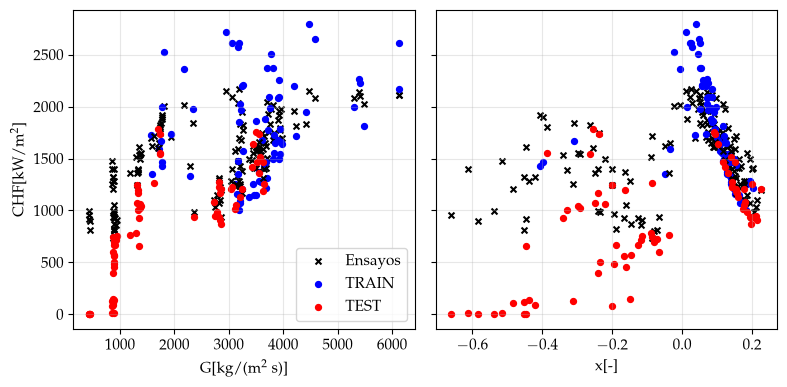
\includegraphics[width=\textwidth]{Figures/chf_lfdnn_gx_caso_mal.png}
    \caption{Relación del CHF predicho con el flujo másico y el título, según el punto predicho por el modelo \texttt{LFDNN} \#4. TRAIN y TEST son los conjuntos de entrenamiento y evaluación correspondientes a la \texttt{HFDNN}, divididos tal que en evaluación se tienen los ensayos de menor flujo másico.}
    \label{fig:lfdnn_chf_gx}
\end{figure}

Para solventar esta dificultad del modelo en la zona subenfriada se propuso una condición de monotonicidad negativa de la derivada del CHF respecto del título termodinámico, es decir, un modelo de PINN para la \lfdnn{}, que se denota \lfpinn{}. Esta incorporación se realizó al modificar el cálculo de la función de pérdida, según la ecuación \ref{eq:lfpinn_loss},
\begin{equation}
    \mathcal{L} = \mathrm{MSE}(\log \mathrm{CHF}) \;+\; \lambda \cdot \frac{1}{\sum w}\sum_i \left[w_i\,\mathrm{ReLU}\!\left(\frac{\partial \log \mathrm{CHF}}{\partial x}\Big|_i\right)\right]^2.
    \label{eq:lfpinn_loss} 
\end{equation}
Los términos $w$ y $w_i$ representan la máscara aplicada por la condición de monotonicidad sobre los puntos de colocación, según en qué región del dominio de las variables de entrada se debe aplicar. En particular, en este caso se diseñó el conjunto de puntos de colocación para la región subenfriada, con valores de presión y $\nicefrac{L}{D_h}$ en los rangos de los ensayos de COBRA3-CP. El término $\lambda$ es el peso atribuido a la condición de monotonicidad. 

\begin{figure}[h]
    \centering
    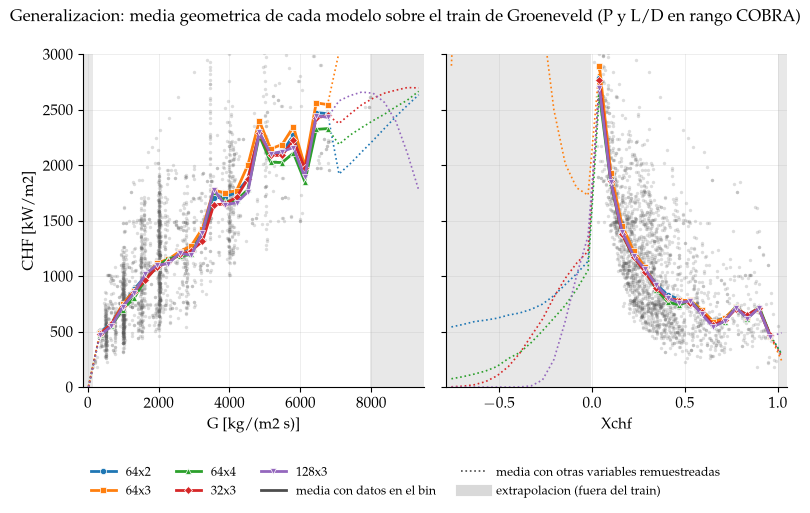
\includegraphics[width=\textwidth]{Figures/chf_lfdnn_generalizacion.png}
    \caption{Evaluación de la generalización de la \lfdnn{} respecto del flujo másico y el título termodinámico.}
    \label{fig:lfdnn_chf_generalizacion}
\end{figure}


Se analizó el impacto de esta implementación en una arquitectura de $64\times 3$, con la misma metodología que las arquitecturas anteriores. Se entrenaron tres redes, variando el valor de $\lambda$ entre $0.01$, $0.1$ y $1$. Esto permite evaluar el impacto del grado en que se impone esta condición frente a los datos.
En la tabla \ref{tab:lfdnn_arqs_comparativa} se presenta la comparativa de las métricas estadísticas sobre los conjuntos de ensayos en un tubo. Esto permite verificar que la condición agregada no perjudica al modelo dentro del conjunto que busca representar.
Se obtiene que los modelos mantienen su precisión respecto de los ensayos de un tubo. La diferencia en RMSE es de menos del $2\%$ respecto del modelo base, lo que indica que la incorporación de la monotonicidad no corrompe el modelo.

\begin{table}[h]
	\centering
	\caption{Arquitecturas de \texttt{LFDNN} propuestas y métricas sobre conjuntos de entrenamiento y evaluación de ensayos en un tubo.}
	\begin{tabular}{c c c c c c} 
        \toprule
        \multirow{2}{*}{\textbf{Arquitectura}} & \multirow{2}{*}{$\bm{\lambda}$} & \multicolumn{2}{c}{\textbf{Entrenamiento}} & \multicolumn{2}{c}{\textbf{Evaluación}} \\
        & & $\mathbf{R^2}$ & \textbf{RMSE} & $\mathbf{R^2}$ & \textbf{RMSE} \\ \hline
        Base                    & -      & $0.9657$ & $296.1$ & $0.9657$ & $294.3$ ($+4.2\%$) \\
        \multirow{3}{*}{PINN}   & $0.01$ & $0.9624$ & $310.0$ & $0.9642$ & $300.9$ ($+4.1\%$) \\
                                & $0.1$  & $0.9638$ & $304.1$ & $0.9652$ & $296.8$ ($+4.7\%$) \\
                                & $1$    & $0.9637$ & $304.6$ & $0.9650$ & $297.6$ ($+5.1\%$) \\
		\bottomrule
	\end{tabular}
	\label{tab:lfdnn_arqs_comparativa}
\end{table}

% Groeneveld                --- log CHF ---                  --- CHF [kW/m2] ---        
% modelo             R2 tr   R2 te  RMSE tr  RMSE te   R2 tr   R2 te   RMSE tr   RMSE te
% --------------------------------------------------------------------------------------
% $\lambda$ = 0     0.9665  0.9632   0.1464   0.1530  0.9605  0.9626     317.5     307.4
% $\lambda$ = 0.01  0.9661  0.9630   0.1473   0.1533  0.9624  0.9642     310.0     300.9
% $\lambda$ = 0.1   0.9661  0.9626   0.1473   0.1542  0.9638  0.9652     304.1     296.8
% $\lambda$ = 1     0.9658  0.9620   0.1479   0.1554  0.9637  0.9650     304.6     297.6

% mejor R2 en test (log):   $\lambda$ = 0  (0.9632)
% mejor RMSE en test (log): $\lambda$ = 0  (0.1530)

% brecha train->test (RMSE en log):
%   $\lambda$ = 0    +0.0066 (+4.5%)
%   $\lambda$ = 0.01 +0.0060 (+4.1%)
%   $\lambda$ = 0.1  +0.0069 (+4.7%)
%   $\lambda$ = 1    +0.0076 (+5.1%)

% costo respecto de lambda = 0 (RMSE en log, test):
%   $\lambda$ = 0    +0.00%
%   $\lambda$ = 0.01 +0.20%
%   $\lambda$ = 0.1  +0.80%
%   $\lambda$ = 1    +1.61%


Luego, en la tabla \ref{tab:lfdnn_dnbrmin_comp}, se comparan los valores de media y desvío estándar del DNBR, el $\mathrm{DNBR}_\mathrm{min}$ y los puntos predichos en la región de entrada y en subcanales interiores. Se obtiene una mejora considerable en todos los modelos PINN, lo que indica que la condición aplicada beneficia al modelo en condiciones subenfriadas. Los valores de DNBR quedan prácticamente centrados y su desvío estándar se redujo a la mitad. En cuanto al $\mathrm{DNBR}_\mathrm{min}$, no se obtuvo una mejora, pero esto se debe a su método de cálculo y a la subpredicción no física del DNBR con el modelo base. La cantidad de predicciones en la región de entrada se reduce de casi el $50\%$ de los ensayos a menos del $7\%$. En cuanto a las predicciones en subcanales internos, se obtiene un aumento, aunque se mantiene en menos de $15\%$ de los ensayos. La conclusión es que la aplicación de la monotonicidad mejora la generalización del modelo a la aplicación de interés.

\begin{table}[H]
	\centering
	\caption{Arquitecturas de \texttt{LFDNN} propuestas y métricas sobre ensayos de bundle de la \cna{}.}
	\begin{tabular}{c c c c c c c} 
        \toprule
        \textbf{Arq.} & $\bm{\lambda}$ & $\bm{\overline{\mathrm{DNBR}}}$ & $\bm{\sigma(\mathrm{DNBR})}$ &  $\bm{\mathrm{DNBR}_\mathrm{min}}$ & \textbf{Z entrada} & \textbf{SCH int.} \\ \hline
        Base    & -      & $0.687$ & $0.403$ & $1.442$ & 72 & 6  \\
        \multirow{3}{*}{PINN} 
                & $0.01$ & $1.061$ & $0.219$ & $1.470$ & 10 & 14 \\
                & $0.1$  & $1.035$ & $0.226$ & $1.457$ & 4  & 14 \\
                & $1$    & $1.037$ & $0.224$ & $1.456$ & 3  & 22 \\
		\bottomrule
	\end{tabular}
	\label{tab:lfdnn_dnbrmin_comp}
\end{table}

Se mantuvo el criterio empleado para evaluar la predicción de los modelos base y se graficó la relación del CHF predicho con el flujo másico y el título termodinámico para el modelo \lfpinn{} con $\lambda=0.1$ en la figura \ref{fig:lfdnn_chf_gx_mon}. Se observa que se predicen unos pocos casos de CHF en región subenfriada, lo que indica una mejora considerable del modelo respecto de su versión base. Adicionalmente, no se observan valores de CHF que tiendan a $0$, como en la figura \ref{fig:lfdnn_chf_gx}.
Luego, en la figura \ref{fig:lfdnn_chf_generalizacion_mono}, se presenta la evaluación de la generalización del modelo respecto del flujo másico y el título termodinámico. Se observa que el modelo ahora presenta un aumento del CHF al reducir el título termodinámico en condiciones subenfriadas. Este es el resultado esperado, reforzado por la monotonicidad aplicada. Se observa una reducción del CHF predicho en la región cercana a $x=0$, lo que se debe a los ensayos disponibles en un tubo para condiciones subenfriadas. Se halló que se tienen unos pocos ensayos de un tubo en condiciones subenfriadas, pero con longitud calefaccionada muy por debajo de las de aplicación en este trabajo. Su efecto queda compensado por la condición de monotonicidad y los puntos de colocación durante el entrenamiento. Una posible mejora a futuro es realizar un filtrado del conjunto de ensayos de Groeneveld para que las variables estén en el rango de aplicación final.

\begin{figure}[H]
    \centering
    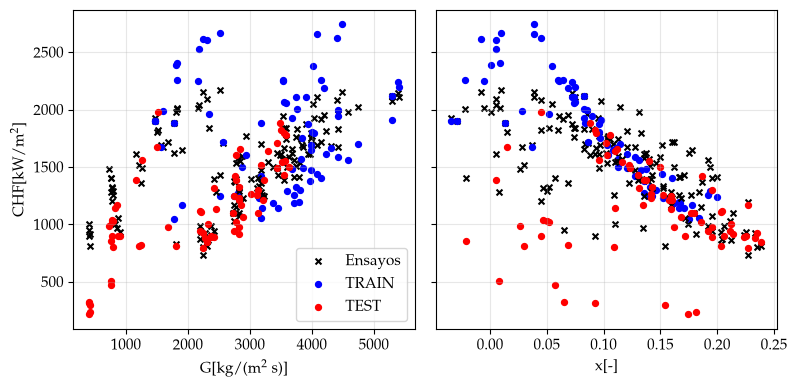
\includegraphics[width=\textwidth]{Figures/chf_lfdnn_gx_mon.png}
    \caption{Relación del CHF predicho con el flujo másico y el título, según el punto predicho por el modelo \texttt{LFDNN} con monotonicidad con $\lambda=0.1$. TRAIN y TEST son los conjuntos de entrenamiento y evaluación correspondientes a la \texttt{HFDNN}, divididos tal que en evaluación se tienen los ensayos de menor flujo másico.}
    \label{fig:lfdnn_chf_gx_mon}
\end{figure}


\begin{figure}[H]
    \centering
    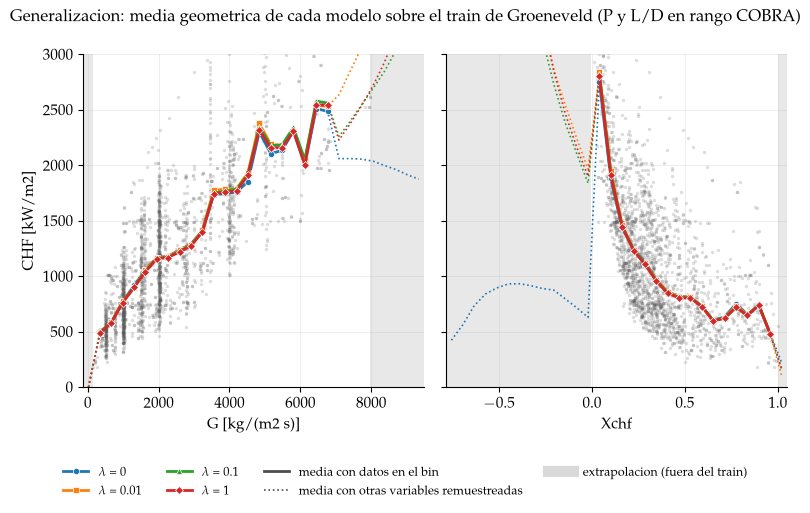
\includegraphics[width=\textwidth]{Figures/chf_lfdnn_generalizacion_mono.png}
    \caption{Evaluación de la generalización de la \lfpinn{} respecto del flujo másico y el título termodinámico, según $\lambda$.}
    \label{fig:lfdnn_chf_generalizacion_mono}
\end{figure}

Por último, en la figura \ref{fig:lfdnn_chf_pred_mono} se grafica el CHF predicho contra medido y el DNBR en cada ensayo para el modelo con $\lambda=0.1$. Se observa una predicción centrada, con algunos outliers en el conjunto de evaluación. Estos casos son los que están por fuera del rango de los ensayos en un tubo, y la red debe extrapolar para estimar CHF. A excepción de estos casos, la predicción del modelo se encuentra contenida en el mismo rango que la metodología actual propuesta por INVAP, que, además de la LUT de Groeneveld, recurre a factores de centrado y corrección desarrollados específicamente para lograr una mejor estimación del CHF en el bundle de la \cna{}, descriptos en la sección \ref{sec:app_tmf}. Esto denota que el modelo de baja fidelidad logra ya una precisión incluso comparable a la metodología actual, sin haber utilizado datos de los ensayos en la geometría específica. 

\begin{figure}[H]
    \centering
    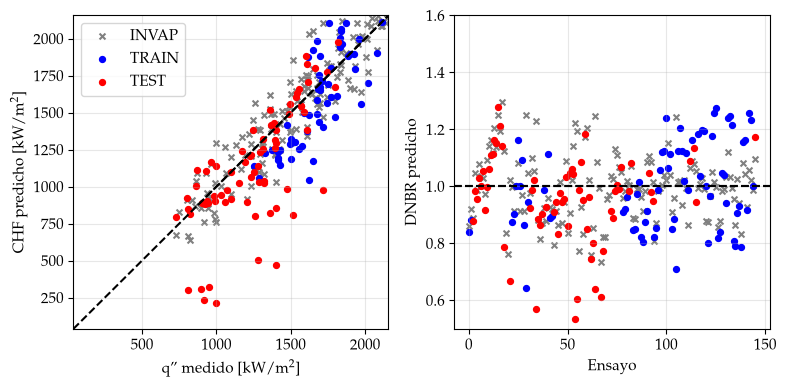
\includegraphics[width=\textwidth]{Figures/chf_lfdnn_pred_mono.png}
    \caption{Predicción de CHF contra medido y $\mathrm{DNBR}$ para cada ensayo, para modelo \lfpinn{} con $\lambda=0.1$.}
    \label{fig:lfdnn_chf_pred_mono}
\end{figure}

\newpage
\subsection{Análisis de arquitectura de multifidelidad}
\label{sec:chf_arq_mfdnn}
Para realizar el análisis de la arquitectura del modelo, se planteó separar la aplicación de multifidelidad de la de información física. En esta sección se estudió el efecto de la primera. Solo se utilizaron las variables base, tradicionales en la predicción de CHF por las LUT de Groeneveld y adoptadas por la \lfpinn{}.
Estas son el flujo másico, la presión, el título termodinámico y la relación de largo calefaccionado con diámetro hidráulico. Las primeras tres son las variables necesarias para interpolar dentro de la LUT, mientras que la cuarta permite transformar la predicción a la geometría de bundle. Groeneveld propone factores de corrección que utilizan algunas de las variables adicionales incorporadas en este trabajo. Para más detalles, ver el apéndice \ref{appendix_groeneveld}.

Las arquitecturas comparadas son las siguientes:
\begin{itemize}
    \item DNN tradicional entrenada directamente sobre las simulaciones con \break\mbox{COBRA3-CP} de los ensayos de la Universidad de Columbia. Constituye un baseline para determinar si las arquitecturas más complejas conllevan una mejora de precisión. También debe evaluarse su comportamiento en regiones no entrenadas y ponerse en tela de juicio si sus predicciones tienen sustento físico.
    % \item DNN tradicional, entrenada directamente sobre las simulaciones con \nobreak COBRA3-CP de los ensayos de la Universidad de Columbia.
    \item \lfpinn{} entrenada sobre los ensayos en un tubo utilizados para conformar las LUT 2006 de Groeneveld. Esto permite tener un baseline del aporte de la predicción de CHF en un tubo y de su contribución a la arquitectura de multifidelidad.
    \item \mfdnn{}, conjunción de la \lfpinn{} y la \hfdnn{}. Esta última fue entrenada sobre las simulaciones de COBRA3-CP de los ensayos de la Universidad de Columbia, con la predicción de la \lfpinn{} como entrada adicional.
    % \item \texttt{MFPINN}, igual a la \texttt{MFDNN}, pero con la aplicación de las relaciones físicas descriptas en la sección \ref{sec:chf_arq}.
\end{itemize}

Para lograr una evaluación que no se limitara a la capacidad de los modelos de representar la información con la que fueron entrenados, se planteó entrenarlos con los casos menos exigentes desde el punto de vista del CHF. Entonces, para dividir entre los conjuntos de entrenamiento y prueba, se utilizaron en entrenamiento aquellos ensayos con un flujo másico superior a $4\,000\,\nicefrac{\mathrm{kg}}{\mathrm{m}^2\mathrm{s}}$. La división se grafica en la figura \ref{fig:chf_div_train_test}. Además del flujo másico, la división se presenta contra el título termodinámico, donde se observa que la división también implica dejar en evaluación a la mayoría de los ensayos que presentaron CHF a título alto. Esto permite evaluar el funcionamiento del modelo al extrapolar hacia condiciones más exigentes de CHF, de forma similar a lo realizado para evaluar y definir la \lfpinn{}.

\begin{figure}[H]
    \centering
    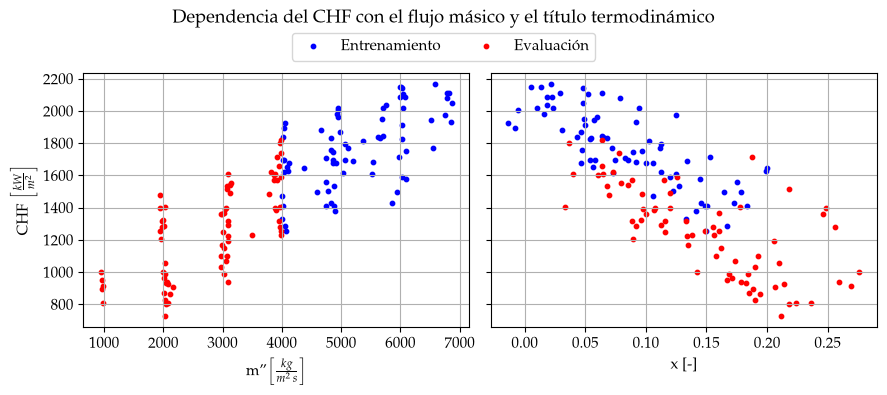
\includegraphics[width=\textwidth]{Figures/chf_division_train_test.png}
    \caption{División de los datos de CHF de la Universidad de Columbia en entrenamiento y evaluación, según flujo másico. Los ejes de flujo másico y título termodinámico corresponden a los valores promedio de la sección de ensayo a la salida.}
    \label{fig:chf_div_train_test}
\end{figure}

Para evitar que los resultados de los modelos evaluados dependan del proceso estocástico de entrenamiento, se entrenaron 50 instancias de cada modelo. De esta forma, se comparan las métricas estadísticas y de $\mathrm{DNBR}$ medias de cada modelo.
Las arquitecturas se evaluaron en su predicción de CHF de forma tradicional, y adicionalmente por medio del $\mathrm{DNBR}_\mathrm{min}$, según lo explicado en la sección \ref{sec:chf_eval}. En la tabla \ref{tab:mf_estadistica} se comparan los valores de $\mathrm{R}^2$ y de RMSE para la DNN, la \lfpinn{} y la \mfdnn{}. 
Se obtuvo un mejor rendimiento por parte de la \mfdnn{} respecto de la DNN en evaluación y muy similar en entrenamiento. En cuanto a la \lfpinn{}, su comportamiento es pobre, con un $\mathrm{R}^2<0$ que indica que una predicción constante e igual a la media obtendría un mejor ajuste.

\begin{table}[h]
	\centering
	\caption{Evaluación por métricas estadísticas de la predicción sobre el conjunto de ensayos de la Universidad de Columbia. Para DNN y \mfdnn{} representa la mediana de 50 redes entrenadas.}
	\begin{tabular}{p{2cm} l c c} 
        \toprule
        \textbf{Modelo} & \textbf{Conjunto} & $\bm{\mathrm{R}^2}$ & $\bm{\mathrm{RMSE}}$ \\ \hline
        \multirow{2}{*}{DNN}     
                & Entrenamiento & $0.951$ & $51.74$ \\
                & Evaluación    & $0.807$ & $121.59$ \\
        \multirow{2}{=}{\lfpinn{} $\lambda=0.1$}     
                & Entrenamiento & $-1.421$ & $365.39$ \\
                & Evaluación    & $-0.221$ & $305.64$ \\
        \multirow{2}{*}{\mfdnn{}}     
                & Entrenamiento & $0.945$ & $54.80$ \\
                & Evaluación    & $0.846$ & $108.67$ \\
		\bottomrule
	\end{tabular}
	\label{tab:mf_estadistica}
\end{table}

En la tabla \ref{tab:mf_dnbr} se comparan, para los mismos modelos, el factor de centrado, la media y el desvío estándar del DNBR y el $\mathrm{DNBR}_\mathrm{min}$. Es importante aclarar que el factor de centrado se calculó en función del conjunto de entrenamiento y luego se aplicó al conjunto de evaluación. De esta forma se tiene un cómputo análogo al que se realiza en inferencia. 
Se obtiene nuevamente un comportamiento similar entre el modelo DNN y \mfdnn{}, con una leve ventaja para este último en evaluación. El desvío estándar en ambos conjuntos es muy similar. En cuanto al modelo \lfpinn{}, los resultados que obtiene son peores en el conjunto de evaluación, producto de que durante su entrenamiento se expuso a menos condiciones similares. Cabe recordar que este modelo fue entrenado con otros conjuntos, correspondientes a ensayos en un tubo. Aun así, al recordar los resultados de la figura \ref{fig:lfdnn_chf_pred_mono}, su comportamiento resulta similar al de la metodología de INVAP, a excepción de entre 10 y 15 puntos en los que se subpredice el CHF.

\begin{table}[H]
	\centering
	\caption{Evaluación por métricas de predicción de $\mathrm{DNBR}$ sobre el conjunto de ensayos de la Universidad de Columbia. Para DNN y \mfdnn{} representa la mediana de 50 redes entrenadas.}
	\begin{tabular}{p{2cm} l c c c c} 
        \toprule
        \textbf{Modelo} & \textbf{Conjunto} & $\bm{f_c}$ & $\bm{\overline{\mathrm{DNBR}}}$ & $\bm{\sigma(\mathrm{DNBR})}$ & $\bm{\mathrm{DNBR}_\mathrm{min}}$ \\ \hline
        \multirow{2}{*}{DNN}     
                & Entrenamiento & \multirow{2}{*}{$1.035$}
                                        & $1.000$ & $0.031$ & $1.060$ \\
                & Evaluación    &       & $1.063$ & $0.109$ & $1.265$ \\
        \multirow{2}{=}{\lfpinn{} $\lambda=0.1$}     
                & Entrenamiento & \multirow{2}{*}{0.916}
                                        & $1.000$ & $0.152$ & $1.300$ \\
                & Evaluación    &       & $0.895$ & $0.240$ & $1.369$ \\
        \multirow{2}{*}{\mfdnn{}}     
                & Entrenamiento & \multirow{2}{*}{$1.003$}
                                        & $1.000$ & $0.032$ & $1.062$ \\
                & Evaluación    &       & $1.041$ & $0.103$ & $1.233$ \\
        % \multirow{2}{*}{MFPINN}     
        %         & Entrenamiento & \multirow{2}{*}{}
        %                                 &  &  &  \\
        %         & Evaluación    &       &  &  &  \\
		\bottomrule
	\end{tabular}
	\label{tab:mf_dnbr}
\end{table}

Al analizar el desvío estándar en el $\mathrm{DNBR}_\mathrm{min}$ obtenido en evaluación, el modelo DNN obtiene un valor de $0.088$, mientras que el \mfdnn{} $0.008$. Esto indica que este último, por su construcción, tiene una mayor robustez y no depende tanto del proceso estocástico de entrenamiento. Esto se evidencia de forma gráfica en la figura \ref{fig:chf_dnbrmin_dist}, donde se presenta la distribución de densidad de probabilidad de $\mathrm{DNBR}_\mathrm{min}$ de cada modelo, para los conjuntos de entrenamiento y de evaluación. Ambos modelos presentan buen comportamiento en entrenamiento, algo no sorprendente a esta altura del trabajo. En evaluación, los resultados permiten apreciar el impacto de tomar como entrada la predicción informada de la \lfpinn{}. El modelo de DNN tradicional presenta una distribución casi uniforme entre $1.1$ y $1.4$, mientras que el modelo \mfdnn{} presenta una distribución con menor desvío estándar y más concentrada. En particular, para esta aplicación, esto es un rasgo positivo, ya que implica que el modelo debe respetar condiciones de fondo que la aleatoriedad no puede mover, es decir, el modelo busca representar la física.

\begin{figure}[h]
    \centering
    
    % \begin{subfigure}[b]{0.60\textwidth}
    %     \centering
    %     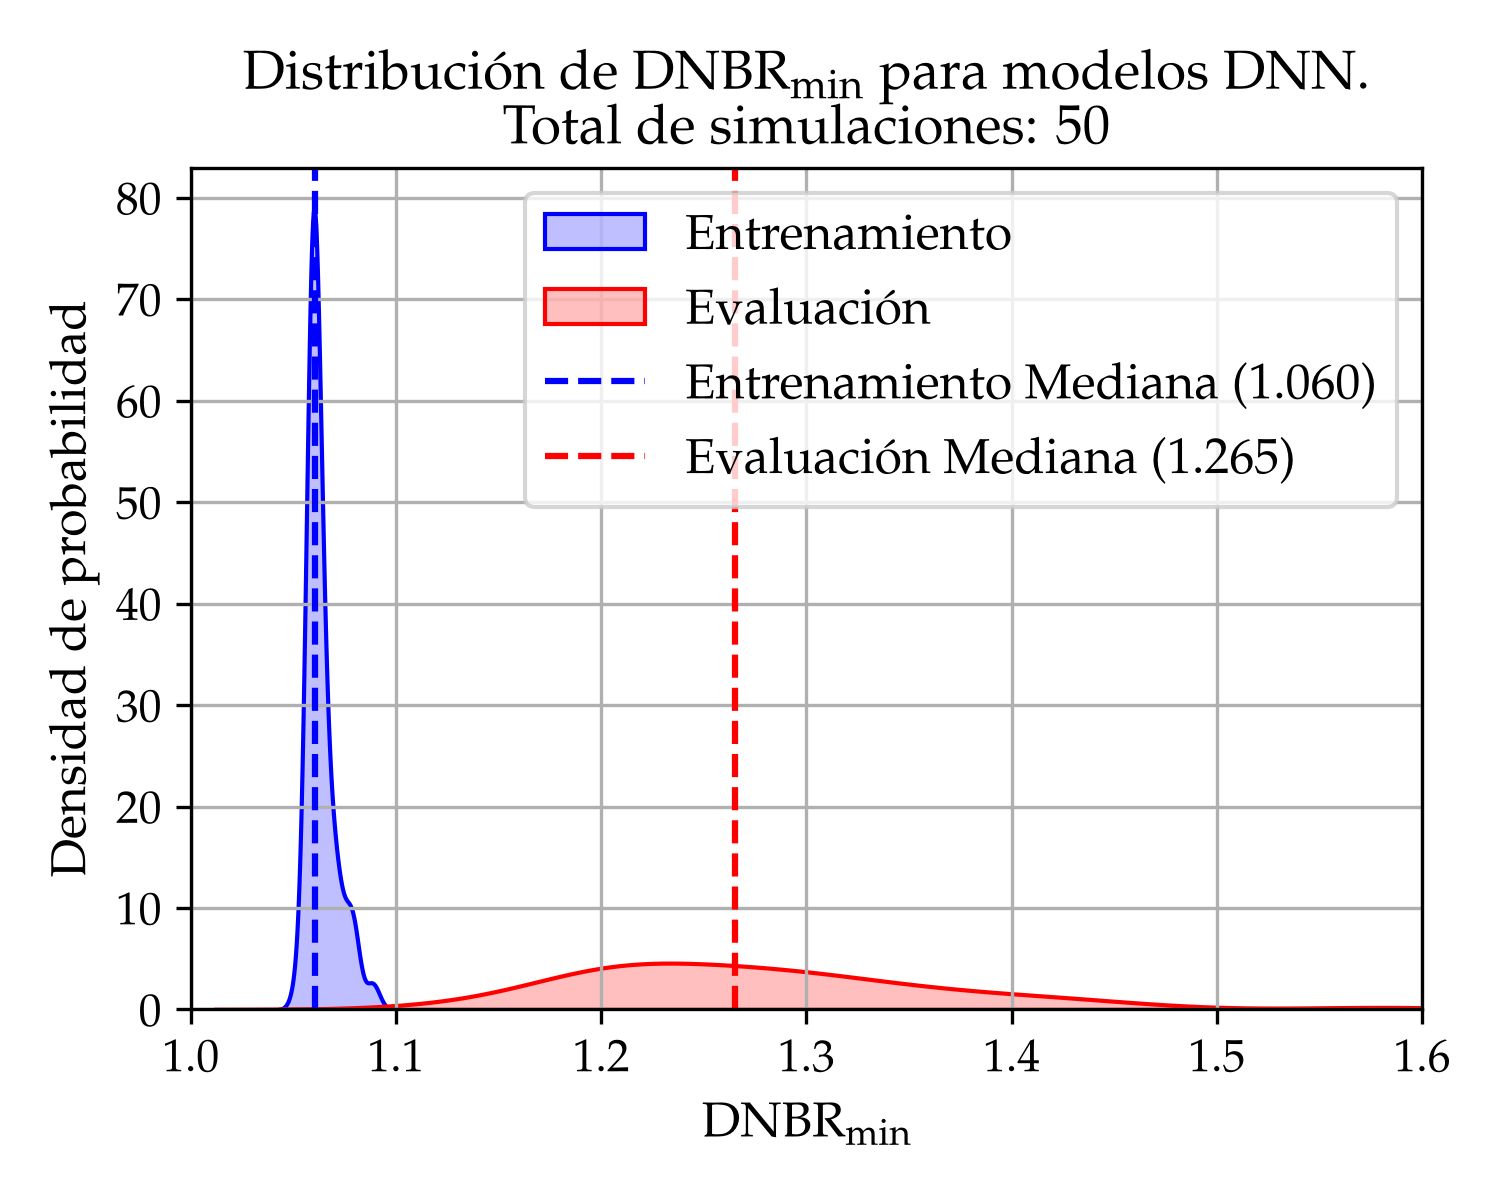
\includegraphics[width=\textwidth]{Figures/chf_distribucion_dnn.png}
    %     \caption{Modelo de DNN tradicional.}
    %     \label{fig:chf_dnbrmin_dist_dnn}
    % \end{subfigure}
    % % \hfill
    % \begin{subfigure}[b]{0.60\textwidth}
    %     \centering
    %     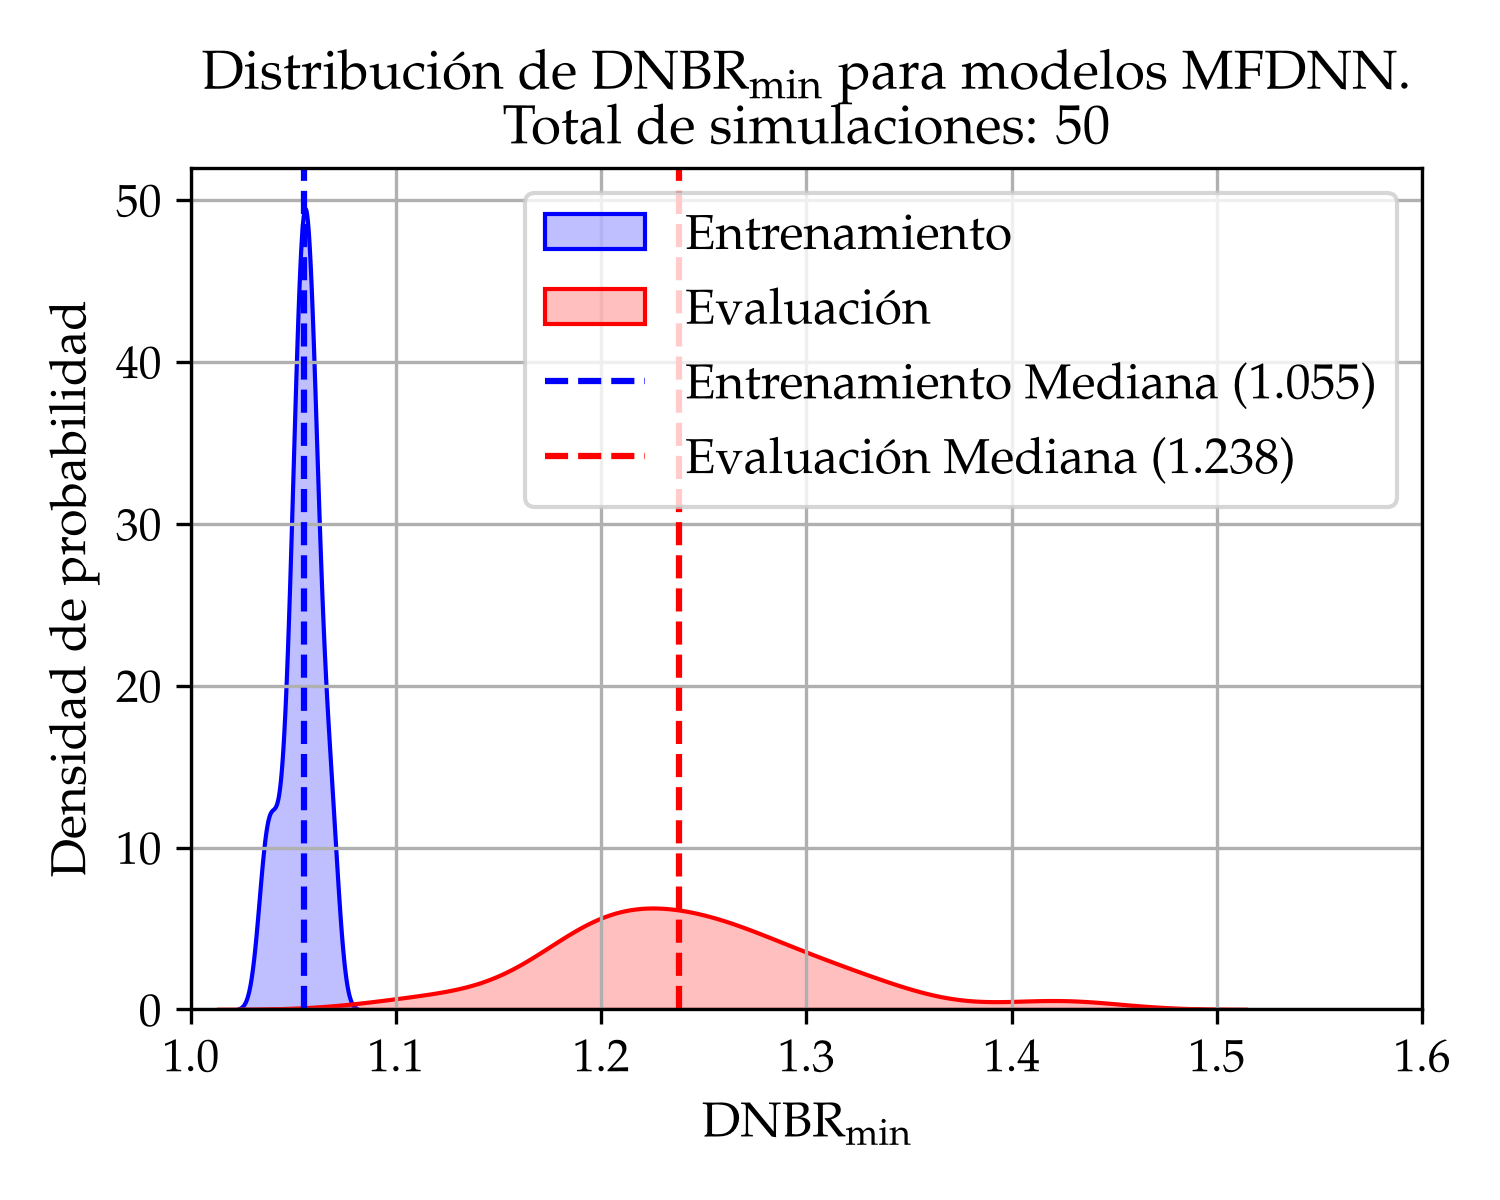
\includegraphics[width=\textwidth]{Figures/chf_distribucion_mfdnn.png}
    %     \caption{Modelo de MFDNN.}
    %     \label{fig:chf_dnbrmin_dist_mfdnn}
    % \end{subfigure}

    \begin{subfigure}[b]{0.48\textwidth}
        \centering
        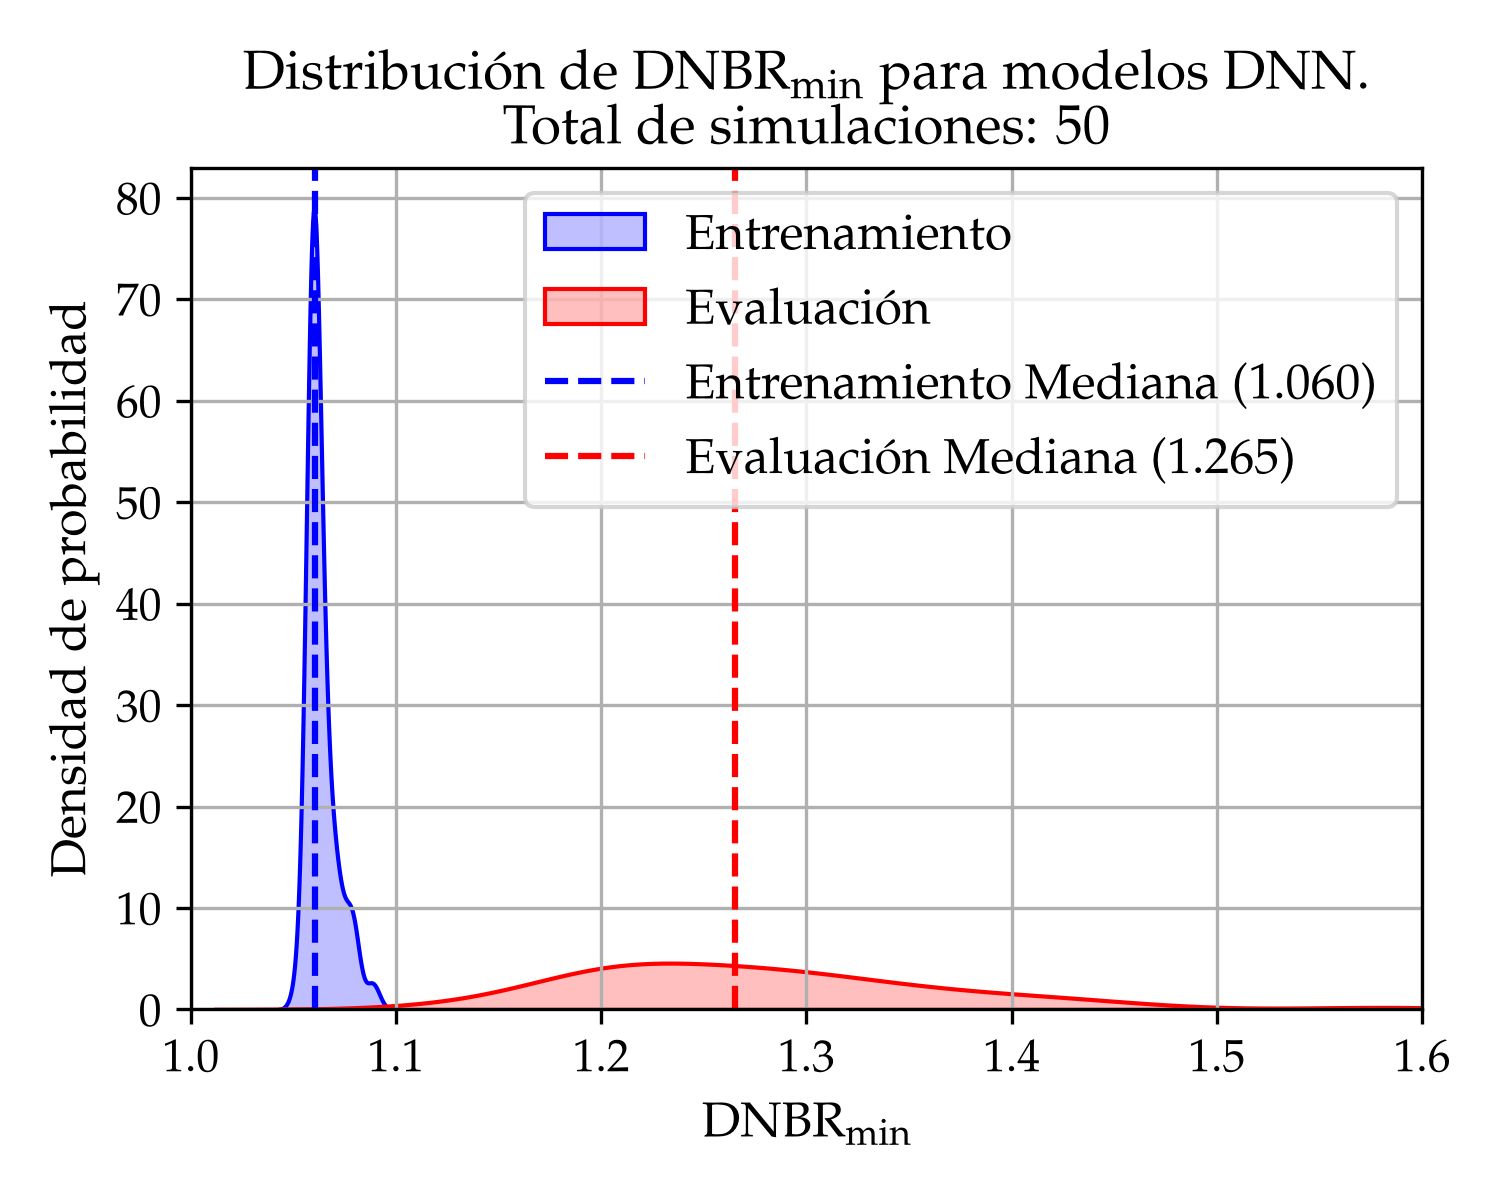
\includegraphics[width=\textwidth]{Figures/chf_distribucion_dnn.png}
        \caption{Modelo de DNN tradicional.}
        \label{fig:chf_dnbrmin_dist_dnn}
    \end{subfigure}
    \hfill
    \begin{subfigure}[b]{0.48\textwidth}
        \centering
        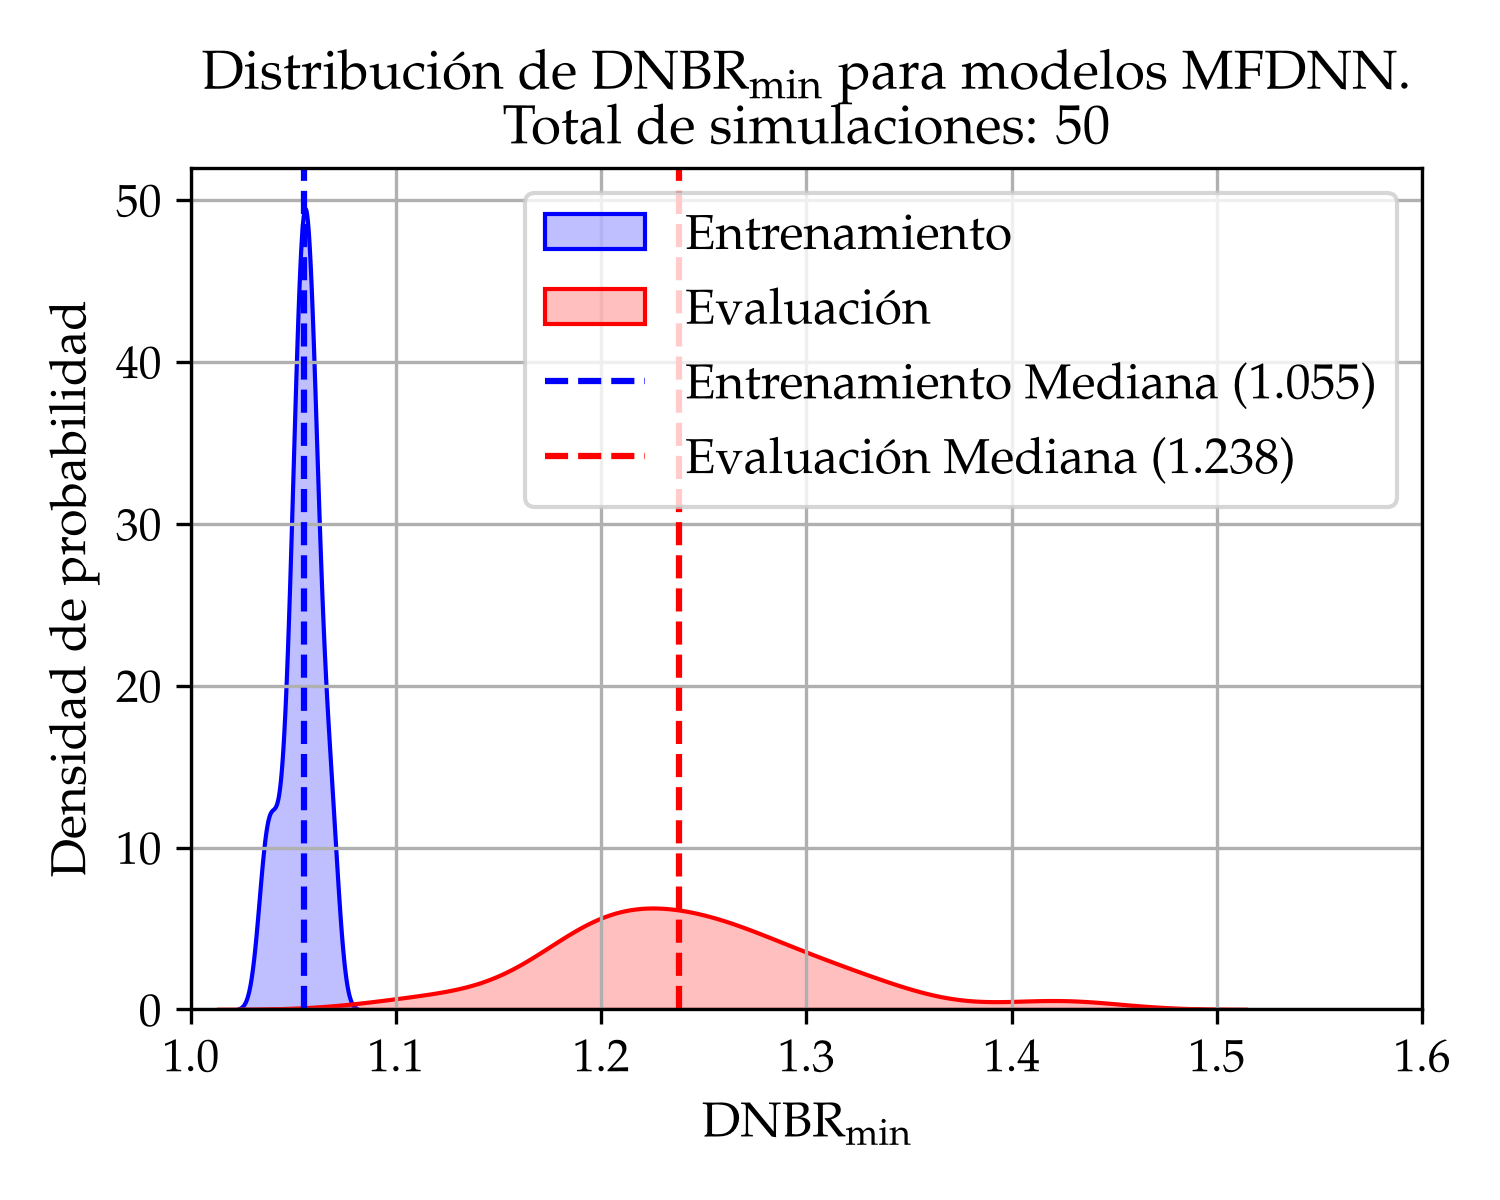
\includegraphics[width=\textwidth]{Figures/chf_distribucion_mfdnn.png}
        \caption{Modelo de MFDNN.}
        \label{fig:chf_dnbrmin_dist_mfdnn}
    \end{subfigure}
    
    \caption{Distribución de probabilidad de $\mathrm{DNBR}_\mathrm{min}$ para \mbox{$N=50$} modelos entrenados de cada tipo.}
    \label{fig:chf_dnbrmin_dist}
\end{figure}

Por último, en la figura \ref{fig:chf_pred_mfnn} se presentan los gráficos de CHF predicho contra medido y de DNBR para cada ensayo, para el modelo con la mediana del $\mathrm{DNBR}_\mathrm{min}$ de entrenamiento de cada variante. El comportamiento de ambos es similar, con una tendencia a subpredecir CHF en algunos casos del conjunto de evaluación. Aun así, se observa que, a excepción de esos puntos extraordinarios, la predicción se encuentra contenida dentro de la de INVAP. Esto indica un mejor comportamiento y destaca el rendimiento de estos modelos aun en condiciones desfavorables de entrenamiento, por no contar con los puntos más limitantes de CHF.

\begin{figure}[h]
    \centering
    
    \begin{subfigure}[b]{\textwidth}
        \centering
        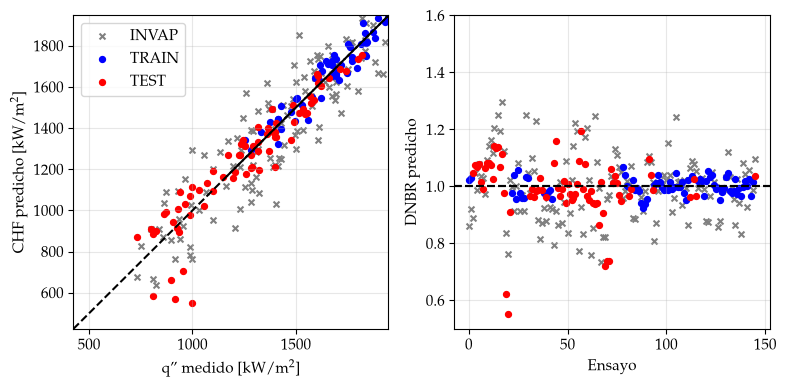
\includegraphics[width=\textwidth]{Figures/chf_dnn_pred.png}
        \caption{Modelo DNN tradicional.}
        \label{fig:chf_pred_dnn}
    \end{subfigure}
    % \hfill
    \begin{subfigure}[b]{\textwidth}
        \centering
        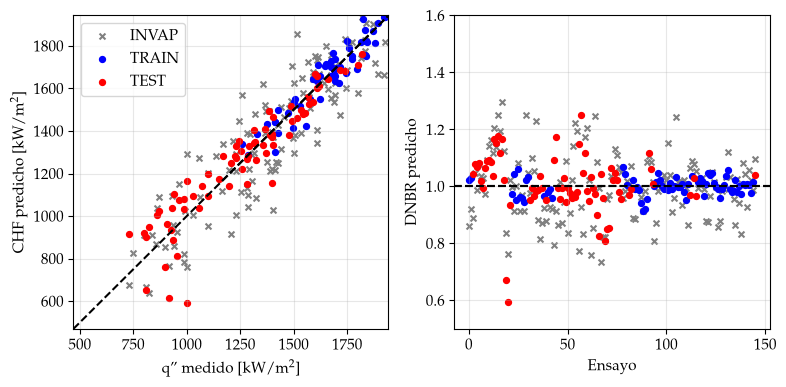
\includegraphics[width=\textwidth]{Figures/chf_mfdnn_pred.png}
        \caption{Modelo \mfdnn{}.}
        \label{fig:chf_pred_mfdnn}
    \end{subfigure}

    \caption{CHF predicho contra medido y DNBR por ensayo para modelos DNN y \mfdnn{}. Se seleccionó para cada variante el modelo con la mediana del $\mathrm{DNBR}_\mathrm{min}$ de entrenamiento.}
    \label{fig:chf_pred_mfnn}
\end{figure}

\subsection{Análisis de arquitectura informada por física}
\label{sec:chf_arq_mfpinn}
Para el análisis de arquitectura informada por física, se adoptó un enfoque de agregación de las condiciones, para poder evaluar el efecto aislado de cada una sobre el modelo. Adicionalmente, se entrenó el modelo con todas las condiciones en conjunto. En la tabla \ref{tab:mfpinn_arqs} se presenta la nomenclatura de las variantes evaluadas. Las variantes A a D fueron planteadas originalmente y, luego, en función de sus resultados, se agregó la variante E al análisis.
El punto de comparación en esta instancia es la red \mfdnn{} evaluada en la sección previa.
Para realizar la comparación se dispuso el entrenamiento de la siguiente forma. Se entrenó una red \mfdnn{} con optimizador Adam durante 500 épocas. De esta forma las redes \mfpinn{} tienen el mismo punto de partida y no dependen fuertemente del proceso estocástico detrás del optimizador para el primer acercamiento a la solución. Luego, se entrenó durante otras 500 épocas cada variante, pero con optimizador L-BFGS, estándar en entrenamiento de redes PINN.

\begin{table}[H]
	\centering
	\caption{Variantes del modelo \mfpinn{} evaluadas.}
	\begin{tabular}{c | C{1cm} | C{1cm} | C{1cm} | C{2cm} | C{2cm}} 
        \toprule
        \multirow{2}{*}{\textbf{Modelo \mfpinn{}}} & \multicolumn{3}{c|}{\textbf{Monotonicidad}} & \multirow{2}{=}{\centering \textbf{Derivada cruzada}} & \multirow{2}{=}{\centering \textbf{Derivada segunda}} \\
        & x & G & p & & \\ \hline
        A & $\blacksquare$ & $\blacksquare$ & $\blacksquare$ & $\blacksquare$ & $\blacksquare$ \\
        B & $\blacksquare$ & $\blacksquare$ & $\blacksquare$ &                &   \\
        B1& $\blacksquare$ &                &                &                &   \\
        B2&                & ${\blacksquare}^{\dagger}$ &                &                &   \\
        B3&                &                & $\blacksquare$ &                &   \\
        C &                &                &                & $\blacksquare$ &   \\
        D &                &                &                &                & $\blacksquare$ \\
        E & $\blacksquare$ & $\blacksquare$ & $\blacksquare$ &                & $\blacksquare$ \\
		\bottomrule
        \multicolumn{6}{l}{
            $\dagger$ \small{Solo se aplica la monotonicidad de G positiva en $(x<0.15)\cup(G<3\,000\,\nicefrac{\mathrm{kg}}{\mathrm{m}^2\mathrm{s}})$.}
        }
	\end{tabular}
	\label{tab:mfpinn_arqs}
\end{table}

En la tabla \ref{tab:mfpinn_arqs_dnbr_train} se compara el rendimiento de los distintos modelos en cuanto a predicción de DNBR en entrenamiento, y en la tabla \ref{tab:mfpinn_arqs_dnbr_test} en evaluación. Nuevamente, el factor de centrado fue calculado sobre el conjunto de entrenamiento y aplicado al de evaluación, de forma análoga a lo que se realiza en inferencia. Se obtiene un rendimiento idéntico entre los modelos en el conjunto de entrenamiento, con una leve mejora respecto del modelo base \mfdnn{}. Esta mejora en todos los modelos es esperable, dado que se dispuso de más épocas de entrenamiento sobre el mismo conjunto.


\begin{table}[h]
	\centering
	\caption{Resultados de predicción de CHF en conjunto de entrenamiento para las arquitecturas evaluadas de \mfpinn{}.}
	\begin{tabular}{c c c c c} 
        \toprule
        \textbf{Modelo} & $f_c$ & $\overline{\mathrm{DNBR}}$ & $\sigma(\mathrm{DNBR})$ & $\mathrm{DNBR}_\mathrm{min}$ \\ \hline
        \mfdnn{}& $1.000$
                                        & $1.000$ & $0.032$ & $1.062$ \\
        A       & $1.000$
                                        & $1.000$ & $0.019$ & $1.037$ \\
        B       & $1.000$
                                        & $1.000$ & $0.021$ & $1.041$ \\
        B1      & $1.000$
                                        & $1.000$ & $0.021$ & $1.042$ \\
        B2      & $1.000$
                                        & $1.000$ & $0.020$ & $1.040$ \\
        B3      & $1.000$
                                        & $1.000$ & $0.023$ & $1.044$ \\
        C       & $1.000$
                                        & $1.000$ & $0.019$ & $1.038$ \\
        D       & $1.000$
                                        & $1.000$ & $0.022$ & $1.044$ \\
        E       & $1.000$
                                        & $1.000$ & $0.020$ & $1.039$ \\
		\bottomrule
	\end{tabular}
	\label{tab:mfpinn_arqs_dnbr_train}
\end{table}

Luego, en evaluación, se obtienen resultados más diversos. Las variantes A, B2 y B3 logran mejorar el rendimiento de la referencia. Se obtuvo un aumento generalizado del desvío estándar y, en los modelos A a B2, una tendencia a subpredecir DNBR, mientras que en los modelos B3 a D se observó una tendencia a sobrepredecir. El modelo E, combinación de los modelos B y D, obtiene una mejora de rendimiento muy cercana a la del modelo completo A. Esta combinación se realizó no en función de los resultados de \dnbrmin{}, sino a partir de los gráficos de CHF predicho contra medido, presentados en las figuras \ref{fig:chf_pred_mfpinn_a}, \ref{fig:chf_pred_mfpinn_b} y \ref{fig:chf_pred_mfpinn_d} para las variantes A, B y D, respectivamente. 
Allí se observa el rendimiento similar entre el modelo completo A y el B, con algunos outliers adicionales en este último, que producen la reducción de rendimiento. Resulta muy interesante el modelo D en la figura \ref{fig:chf_pred_mfpinn_d}, que presenta una distribución muy cercana a la recta unitaria, con tres ensayos de sobrepredicción importante del CHF. Estos tres puntos son los que penalizan fuertemente el resultado de \dnbrmin{} de este modelo. Por este motivo se planteó la combinación de los modelos B y D en el E. Los resultados de CHF predicho contra real se presentan en la figura \ref{fig:chf_pred_mfpinn_e}, donde se observa un rendimiento sin los casos de sobrepredicción de CHF del modelo D y con una nube más cercana a la recta unitaria que el modelo B. En todos los modelos evaluados se obtuvo subpredicción de CHF para los ensayos con menor caudal. Esto se evidencia en las figuras \ref{fig:chf_gx_mfpinn_a}, \ref{fig:chf_gx_mfpinn_b} y \ref{fig:chf_gx_mfpinn_d}, donde se presentan los resultados de CHF en función del flujo másico y el título termodinámico para las variantes A, B y D, respectivamente.

En función de los resultados de esta sección, se definió utilizar la variante E como modelo final \mfpinn{}.

El máximo \dnbrmin{} para \mfdnn{} fue $XXX$ y para \mfpinn{} $XXX$.

\begin{table}[h]
	\centering
	\caption{Resultados de predicción de CHF en conjunto de evaluación para las arquitecturas evaluadas de \mfpinn{}.}
	\begin{tabular}{c c c c c} 
        \toprule
        \textbf{Modelo} & $f_c$ & $\overline{\mathrm{DNBR}}$ & $\sigma(\mathrm{DNBR})$ & $\mathrm{DNBR}_\mathrm{min}$ \\ \hline
        \mfdnn{}& $1.000$
                                        & $1.031$ & $0.094$ & $1.217$ \\
        A       & $1.000$
                                        & $0.965$ & $0.117$ & $1.196$ \\
        B       & $1.000$
                                        & $0.999$ & $0.146$ & $1.289$ \\
        B1       & $1.000$
                                        & $0.939$ & $0.171$ & $1.277$ \\
        B2       & $1.000$
                                        & $0.961$ & $0.124$ & $1.207$ \\
        B3       & $1.000$
                                        & $1.006$ & $0.103$ & $1.210$ \\
        C       & $1.000$
                                        & $1.005$ & $0.217$ & $1.436$ \\
        D       & $1.000$
                                        & $1.028$ & $0.188$ & $1.400$ \\
        E       & $1.000$
                                        & $0.961$ & $0.122$ & $1.203$ \\
		\bottomrule
	\end{tabular}
	\label{tab:mfpinn_arqs_dnbr_test}
\end{table}

\begin{figure}[H]
    \centering
    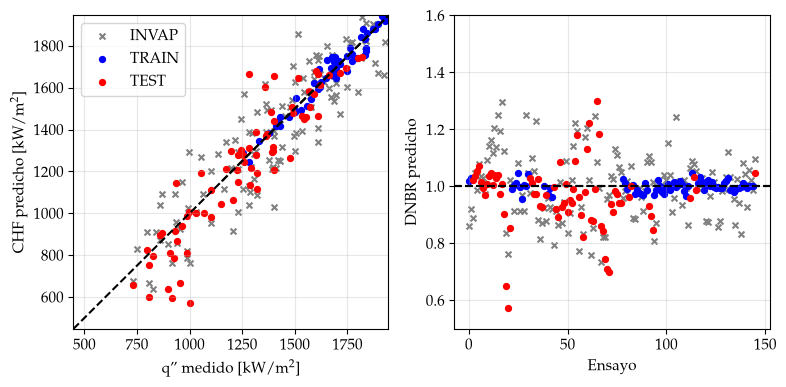
\includegraphics[width=0.95\textwidth]{Figures/chf_mfpinn_A.png}
    \caption{CHF predicho contra medido y DNBR por ensayo para variante A de \mfpinn{}.}
    \label{fig:chf_pred_mfpinn_a}
\end{figure}

\begin{figure}[H]
    \centering
    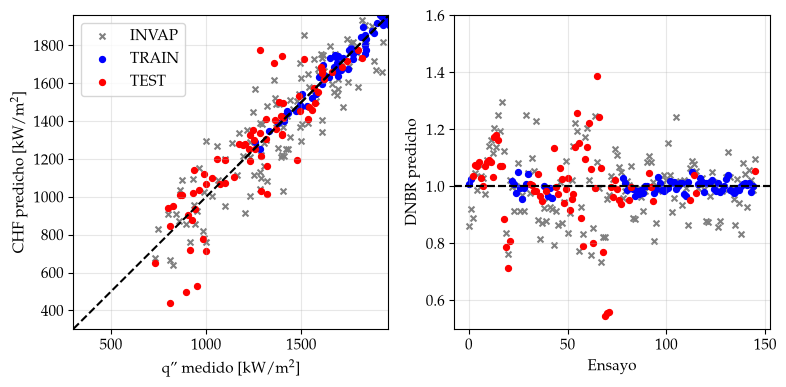
\includegraphics[width=0.95\textwidth]{Figures/chf_mfpinn_B.png}
    \caption{CHF predicho contra medido y DNBR por ensayo para variante B de \mfpinn{}.}
    \label{fig:chf_pred_mfpinn_b}
\end{figure}

\begin{figure}[H]
    \centering
    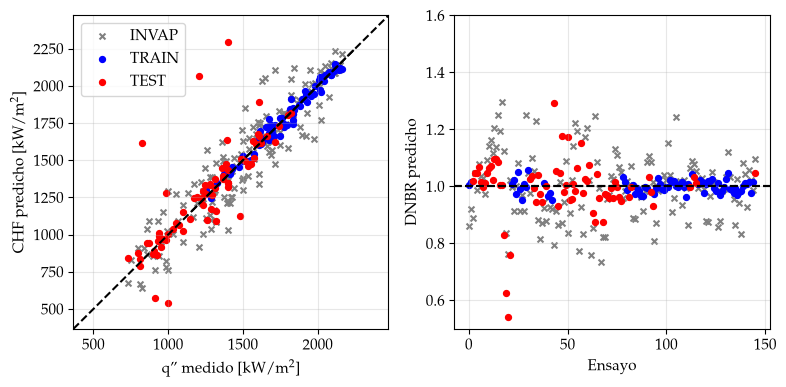
\includegraphics[width=0.95\textwidth]{Figures/chf_mfpinn_D.png}
    \caption{CHF predicho contra medido y DNBR por ensayo para variante D de \mfpinn{}.}
    \label{fig:chf_pred_mfpinn_d}
\end{figure}

% \begin{figure}[h]
%     \centering
    
%     \begin{subfigure}[b]{\textwidth}
%         \centering
%         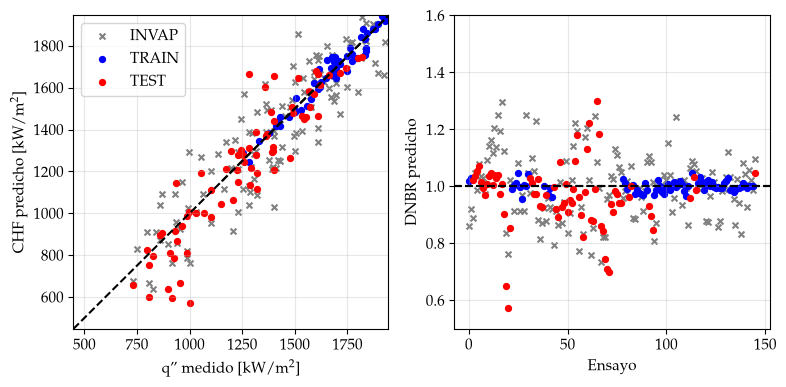
\includegraphics[width=\textwidth]{Figures/chf_mfpinn_A.png}
%         \caption{Variante A.}
%         \label{fig:chf_pred_mfpinn_a}
%     \end{subfigure}
%     % \hfill
%     \begin{subfigure}[b]{\textwidth}
%         \centering
%         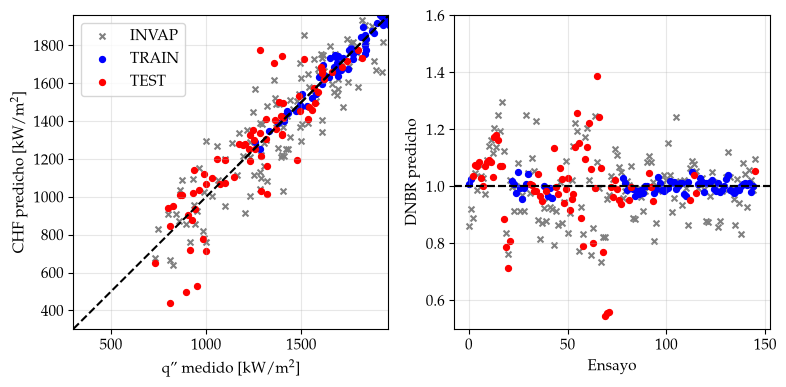
\includegraphics[width=\textwidth]{Figures/chf_mfpinn_B.png}
%         \caption{Variante B}
%         \label{fig:chf_pred_mfpinn_b}
%     \end{subfigure}

%     \begin{subfigure}[b]{\textwidth}
%         \centering
%         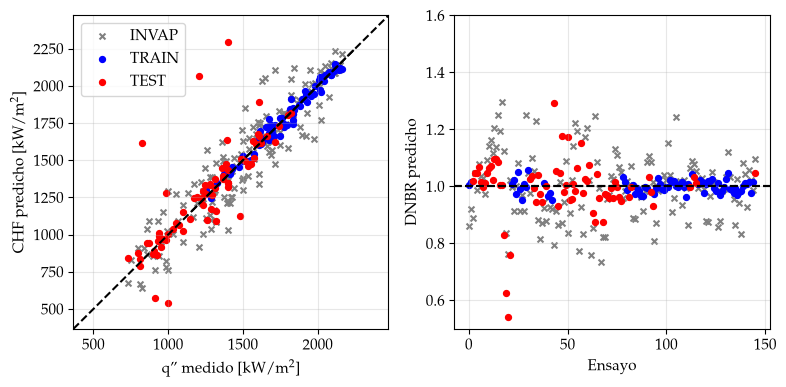
\includegraphics[width=\textwidth]{Figures/chf_mfpinn_D.png}
%         \caption{Variante D.}
%         \label{fig:chf_pred_mfpinn_d}
%     \end{subfigure}

%     \caption{CHF predicho contra medido y DNBR por ensayo para variantes A, B y D de \mfpinn{}.}
%     \label{fig:chf_pred_mfpinn_variantes}
% \end{figure}

\begin{figure}[H]
    \centering
    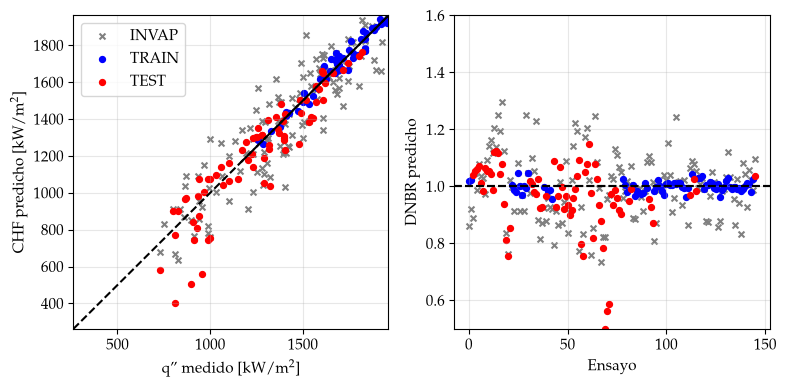
\includegraphics[width=0.95\textwidth]{Figures/chf_mfpinn_E.png}
    \caption{CHF predicho contra medido y DNBR por ensayo para variante E de \mfpinn{}.}
    \label{fig:chf_pred_mfpinn_e}
\end{figure}

% \begin{figure}[H]
%     \centering
    
%     \begin{subfigure}[b]{\textwidth}
%         \centering
%         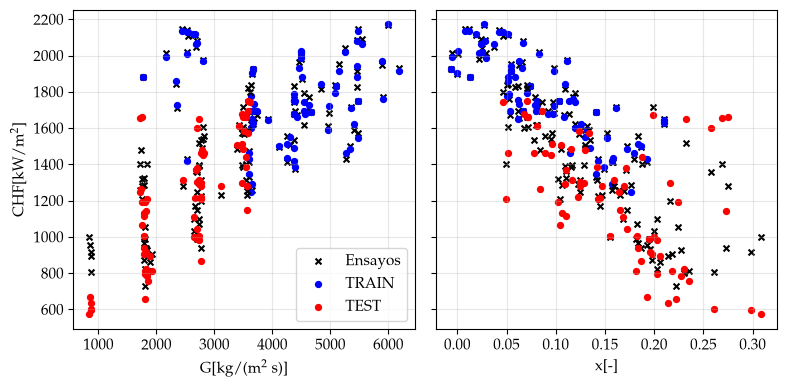
\includegraphics[width=\textwidth]{Figures/chf_mfpinn_gx_A.png}
%         \caption{Variante A.}
%         \label{fig:chf_gx_mfpinn_a}
%     \end{subfigure}
%     % \hfill
%     \begin{subfigure}[b]{\textwidth}
%         \centering
%         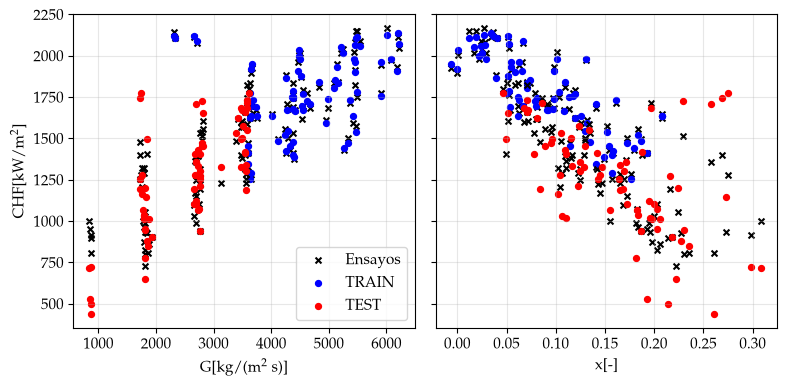
\includegraphics[width=\textwidth]{Figures/chf_mfpinn_gx_B.png}
%         \caption{Variante B}
%         \label{fig:chf_gx_mfpinn_b}
%     \end{subfigure}

%     \begin{subfigure}[b]{\textwidth}
%         \centering
%         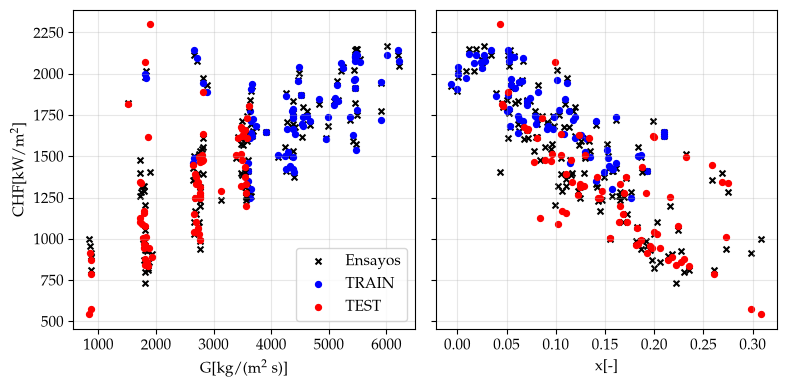
\includegraphics[width=\textwidth]{Figures/chf_mfpinn_gx_D.png}
%         \caption{Variante D.}
%         \label{fig:chf_gx_mfpinn_d}
%     \end{subfigure}

%     \caption{Relación entre CHF predicho y flujo másico y título termodinámico para variantes A, B y D de \mfpinn{}.}
%     \label{fig:chf_gx_mfpinn_variantes}
% \end{figure}

\begin{figure}[H]
    \centering
    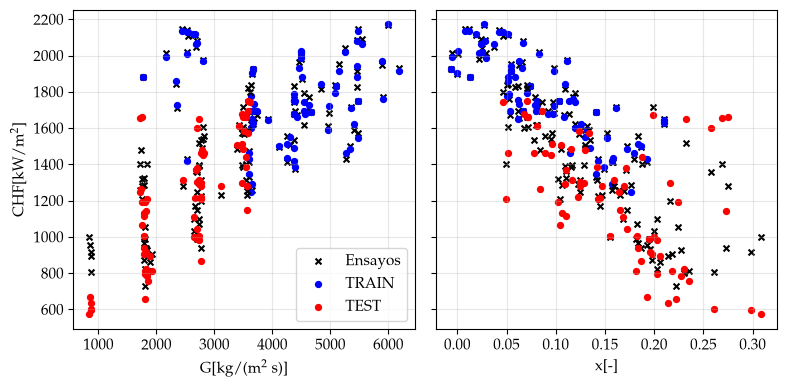
\includegraphics[width=0.95\textwidth]{Figures/chf_mfpinn_gx_A.png}
    \caption{Relación entre CHF predicho y flujo másico y título termodinámico para variante A de \mfpinn{}.}
    \label{fig:chf_gx_mfpinn_a}
\end{figure}

\begin{figure}[H]
    \centering
    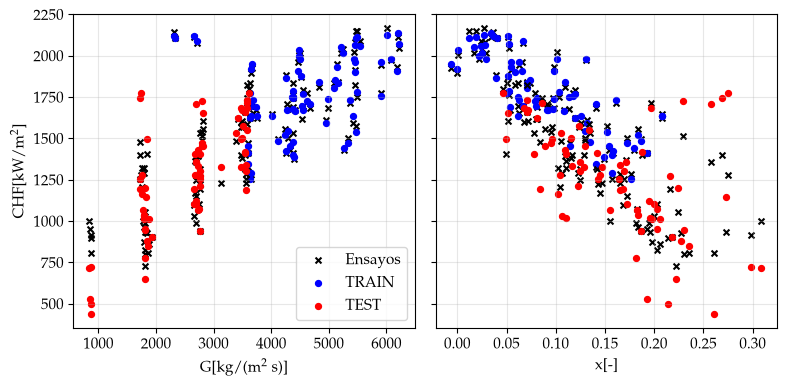
\includegraphics[width=0.95\textwidth]{Figures/chf_mfpinn_gx_B.png}
    \caption{Relación entre CHF predicho y flujo másico y título termodinámico para variante B de \mfpinn{}.}
    \label{fig:chf_gx_mfpinn_b}
\end{figure}

\begin{figure}[H]
    \centering
    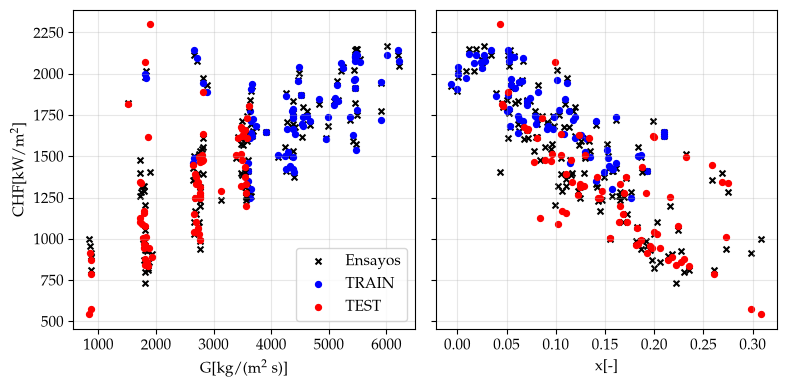
\includegraphics[width=0.95\textwidth]{Figures/chf_mfpinn_gx_D.png}
    \caption{Relación entre CHF predicho y flujo másico y título termodinámico para variante D de \mfpinn{}.}
    \label{fig:chf_gx_mfpinn_d}
\end{figure}


\subsection{Análisis de variables de entrada}
\label{sec:chf_variables_entrada}

Las variables de entrada propuestas en la sección \ref{sec:chf_pipeline} fueron el flujo másico, la presión, el título termodinámico, la relación de largo calefaccionado con diámetro hidráulico, la distancia adimensional al separador aguas arriba, el desbalance de título termodinámico respecto del valor medio del bundle, el factor de pico de potencia y la relación entre perímetro calefaccionado y mojado del subcanal. 
Las primeras cuatro variables son las clásicas utilizadas por la LUT de Groeneveld, y se consideran las más importantes para la predicción de CHF. Las cuatro variables restantes fueron propuestas en este trabajo, y se debe evaluar su contribución al modelo.

Se entrenaron el modelo \mfdnn{} y las variantes A, B, C y D del modelo \mfpinn{}. Al igual que en la sección anterior, para el modelo \mfdnn{} se entrenaron 50 instancias y se informan las medianas de las métricas. En cuanto a las variantes \mfpinn{}, no se realizó un estudio de ese tipo, debido a que su costo de entrenamiento es considerablemente elevado.

En la tabla \ref{tab:mfpinn_exp_dnbr_train} se presentan el factor de centrado, la media y el desvío estándar del DNBR predicho y el \dnbrmin{} para el conjunto de entrenamiento. Se obtuvo un rendimiento similar al del caso con las variables base, levemente mejorado en las variantes \mfpinn{}.

\begin{table}[H]
	\centering
	\caption{Resultados de predicción de CHF en conjunto de entrenamiento para las arquitecturas evaluadas de \mfpinn{}.}
	\begin{tabular}{c c c c c} 
        \toprule
        \textbf{Modelo} & $f_c$ & $\overline{\mathrm{DNBR}}$ & $\sigma(\mathrm{DNBR})$ & $\mathrm{DNBR}_\mathrm{min}$ \\ \hline
        \mfdnn{}    & $1.007$ & $1.000$ & $0.028$ & $1.055$ \\
        \mfpinn{} A & $1.000$ & $1.000$ & $0.010$ & $1.020$ \\
        \mfpinn{} B & $1.000$ & $1.000$ & $0.014$ & $1.028$ \\
        \mfpinn{} D & $1.000$ & $1.000$ & $0.018$ & $1.035$ \\
        \mfpinn{} E & $1.000$ & $1.000$ & $0.013$ & $1.026$ \\
		\bottomrule
	\end{tabular}
	\label{tab:mfpinn_exp_dnbr_train}
\end{table}

En cuanto al conjunto de evaluación, sí se obtuvieron diferencias en el rendimiento respecto de utilizar las variables base. En la tabla \ref{tab:mfpinn_exp_dnbr_test} se presentan las métricas para dicho conjunto. La \mfdnn{} presenta un rendimiento casi idéntico al caso anterior. Las variantes A y E de \mfpinn{} presentaron un rendimiento muy pobre, con un \dnbrmin{} mayor incluso que el de la \lfdnn{}. La variante B presenta una mejora, producto de una reducción del desvío estándar y un aumento en la subpredicción del CHF. 
La variante D presenta un rendimiento sobresaliente, con el mejor \dnbrmin{} obtenido hasta este punto del trabajo. Por ello, se investigó el resultado con mayor detalle, al graficar la relación de los CHF predichos con el flujo másico y el título termodinámico en la figura \ref{fig:chf_mfpinn_d_gx_exp}. Allí se puede ver que el modelo predice CHF en condiciones subenfriadas en múltiples ensayos. Este resultado pone en tela de juicio el sentido físico de estas predicciones.

\begin{table}[H]
	\centering
	\caption{Resultados de predicción de CHF en conjunto de evaluación para las arquitecturas evaluadas de \mfpinn{}.}
	\begin{tabular}{c c c c c} 
        \toprule
        \textbf{Modelo} & $f_c$ & $\overline{\mathrm{DNBR}}$ & $\sigma(\mathrm{DNBR})$ & $\mathrm{DNBR}_\mathrm{min}$ \\ \hline
        \mfdnn{}    & $1.007$ & $1.046$ & $0.097$ & $1.238$ \\
        \mfpinn{} A & $1.000$ & $1.233$ & $0.451$ & $2.125$ \\
        \mfpinn{} B & $1.000$ & $0.953$ & $0.126$ & $1.202$  \\
        \mfpinn{} D & $1.000$ & $0.956$ & $0.089$ & $1.133$  \\
        \mfpinn{} E & $1.000$ & $1.321$ & $0.358$ & $2.030$  \\
		\bottomrule
	\end{tabular}
	\label{tab:mfpinn_exp_dnbr_test}
\end{table}

\begin{figure}[H]
    \centering
    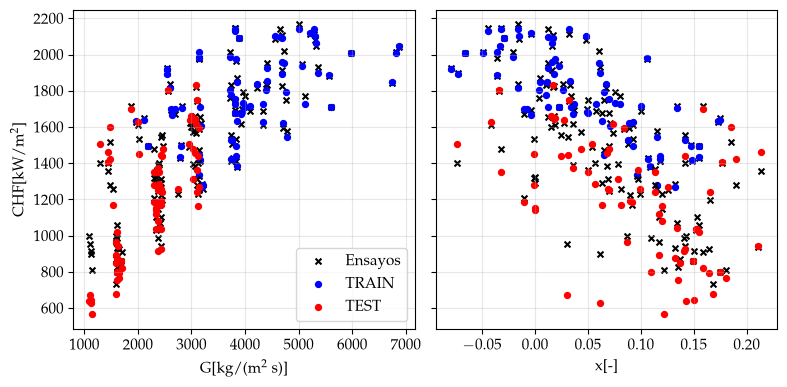
\includegraphics[width=0.95\textwidth]{Figures/chf_mfpinn_gx_D_exp.png}
    \caption{Relación de CHF con el flujo másico y el título termodinámico para variante D de \mfpinn{}, con variables de entrada expandidas.}
    \label{fig:chf_mfpinn_d_gx_exp}
\end{figure}

Se presentan los resultados de CHF predicho contra real y DNBR por ensayo para el modelo \mfdnn{} en la figura \ref{fig:chf_mfdnn_exp} y para la variante E del modelo \mfpinn{} en la figura \ref{fig:chf_mfpinn_exp}. Ambos obtienen una tendencia a la sobrepredicción para el conjunto de evaluación. Para la variante E se observa un rendimiento muy pobre, como lo indican las métricas de DNBR, con una sobrepredicción preocupante del CHF.

\begin{figure}[H]
    \centering
    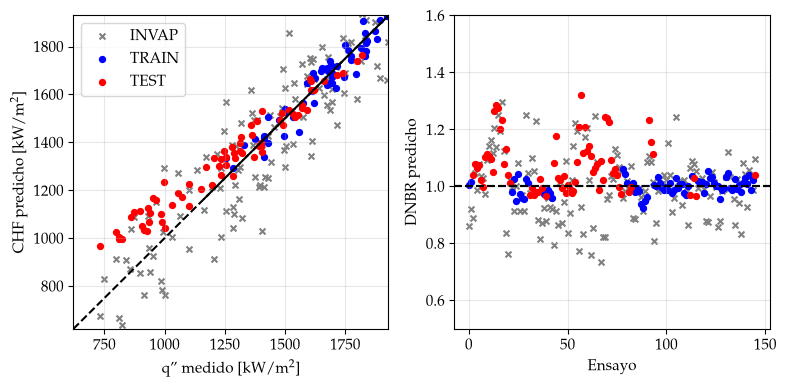
\includegraphics[width=0.95\textwidth]{Figures/chf_mfdnn_pred_exp.png}
    \caption{CHF predicho contra real y DNBR por ensayo, para \mfdnn{} con variables de entrada expandidas.}
    \label{fig:chf_mfdnn_exp}
\end{figure}

\begin{figure}[H]
    \centering
    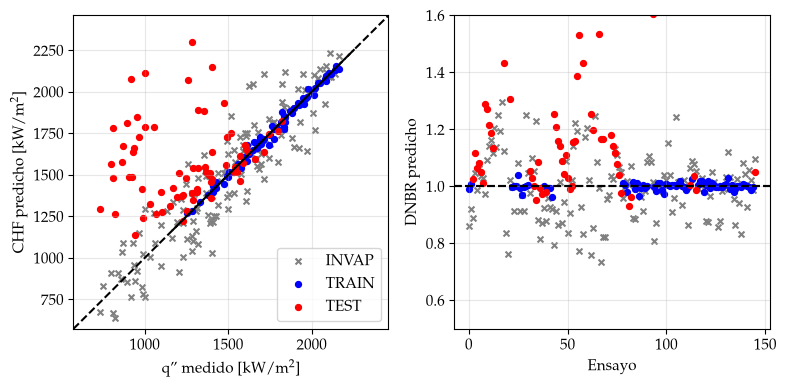
\includegraphics[width=0.95\textwidth]{Figures/chf_mfpinn_E_exp.png}
    \caption{CHF predicho contra real y DNBR por ensayo, para variante E de \mfpinn{} con variables de entrada expandidas.}
    \label{fig:chf_mfpinn_exp}
\end{figure}

La conclusión obtenida es que la inclusión de estas variables en el modelo no representa una mejora clara en las predicciones, e incluso puede resultar en predicciones con tendencias no físicas. Por lo tanto, los modelos finales solo utilizan las variables básicas.


\subsection{Modelos finales}
En las secciones \ref{sec:chf_arq_mfdnn} y \ref{sec:chf_arq_mfpinn} se validó la robustez de los modelos \mfdnn{} y \mfpinn{} para la estimación de CHF al restringir su entrenamiento a condiciones de medio a alto caudal y evaluación a bajo caudal. Dichas condiciones implican una penalización importante al modelo, ya que su conjunto de entrenamiento no contiene datos de las condiciones más críticas para el CHF. Si bien este análisis permitió validar el funcionamiento de los modelos, sus versiones finales no deben tener aplicada esta penalización. Por lo tanto, fueron entrenados con una división aleatoria entre conjuntos de entrenamiento y evaluación, con un 20\% de los datos reservados para evaluación. Se realizó la división con estratificación por conjunto de ensayos de la Universidad de Columbia, de forma de tener datos de los 4 conjuntos de ensayos disponibles.

En la tabla \ref{tab:mf_final_dnbr} se presentan los resultados de las métricas de predicción de $\mathrm{DNBR}$ para \mfdnn{} y \mfpinn{}. Adicionalmente se tienen los valores de la metodología actual, implementada por INVAP. Aquí se puede comparar directamente con ella, ya que los modelos \mfdnn{} y \mfpinn{} fueron entrenados con todo el rango de los ensayos. La metodología actual fue calibrada sin dejar un conjunto de evaluación, por lo que su capacidad de extrapolar por fuera del rango de calibración no ha sido estudiada.

El modelo \mfdnn{} obtiene un rendimiento similar a los análisis previos en el conjunto de entrenamiento, pero en este caso el \dnbrmin{} para evaluación es del mismo orden. La reducción del \dnbrmin{} es considerable respecto de la metodología actual. El modelo \mfpinn{} tiene aún mejor comportamiento, con un \dnbrmin{} en evaluación incluso menor que el de \mfdnn{} en entrenamiento. Adicionalmente, el desvío estándar también se ve reducido para el modelo \mfpinn{}, lo que indica que predice con un error consistentemente bajo.

\begin{table}[H]
	\centering
	\caption{Evaluación por métricas de predicción de $\mathrm{DNBR}$ sobre el conjunto de ensayos de la Universidad de Columbia. Para \mfdnn{} representa la mediana de 50 redes entrenadas. Entrenamiento y evaluación divididos de forma aleatoria.}
	\begin{tabular}{p{2cm} l c c c c} 
        \toprule
        \textbf{Modelo} & \textbf{Conjunto} & $\bm{f_c}$ & $\bm{\overline{\mathrm{DNBR}}}$ & $\bm{\sigma(\mathrm{DNBR})}$ & $\bm{\mathrm{DNBR}_\mathrm{min}}$ \\ \hline
        INVAP   & -           & $1.164$ & $0.999$ & $0.113$ & $1.212$ \\
        \multirow{2}{*}{\mfdnn{}}     
                & Entrenamiento & \multirow{2}{*}{$1.002$}
                                        & $1.000$ & $0.050$ & $1.094$ \\
                & Evaluación    &       & $0.998$ & $0.054$ & $1.113$ \\
        \multirow{2}{*}{\mfpinn{}}     
                & Entrenamiento & \multirow{2}{*}{$1.005$}
                                        & $1.000$ & $0.029$ & $1.056$ \\
                & Evaluación    &       & $0.987$ & $0.044$ & $1.084$ \\
		\bottomrule
	\end{tabular}
	\label{tab:mf_final_dnbr}
\end{table}

En la figura \ref{fig:dist_mfdnn_final} se presenta la distribución de densidad de probabilidad de \dnbrmin{} para los 50 modelos \mfdnn{} entrenados. Nuevamente, se evidencia un rendimiento en evaluación consistente y cercano al de entrenamiento. En la figura \ref{fig:chf_mfdnn_final} se presentan los gráficos de CHF predicho contra real y DNBR por ensayo para el modelo \mfdnn{} con el valor mediano de \dnbrmin{}. Comparado con las predicciones por la metodología INVAP, se obtiene una distribución más centrada en la recta de identidad, y todos los valores de DNBR quedan contenidos aproximadamente entre $0.9$ y $1.1$.

Finalmente, en la figura \ref{fig:chf_mfpinn_final} se presentan para el modelo \mfpinn{} los gráficos de CHF predicho contra real y de DNBR por ensayo. La distribución de predicciones es aún más cercana que la de la \mfdnn{}, lo que refuerza los valores de \dnbrmin{} presentados previamente.

\begin{figure}[H]
    \centering
    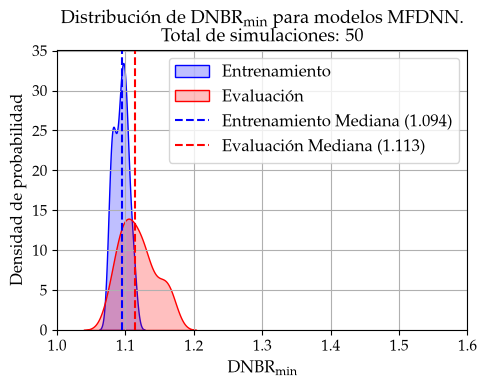
\includegraphics[width=0.6\textwidth]{Figures/chf_distribucion_mfdnn_final.png}
    \caption{Distribución de densidad de probabilidad de \dnbrmin{} para 50 modelos \mfdnn{} entrenados.}
    \label{fig:dist_mfdnn_final}
\end{figure}

\begin{figure}[H]
    \centering
    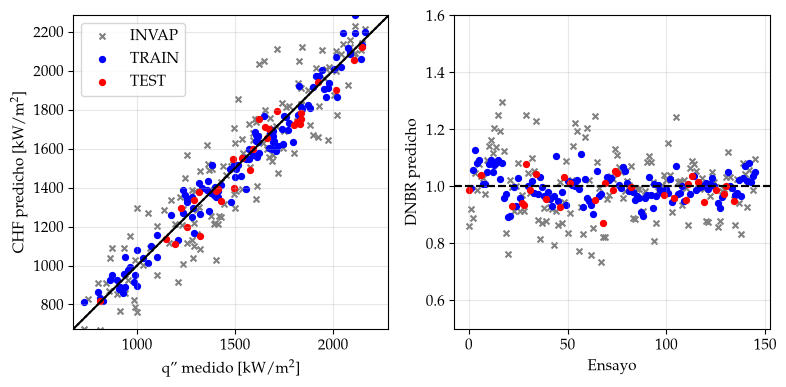
\includegraphics[width=0.95\textwidth]{Figures/chf_mfdnn_pred_final.png}
    \caption{CHF predicho contra real y DNBR por ensayo para modelo final \mfdnn{}.}
    \label{fig:chf_mfdnn_final}
\end{figure}

\begin{figure}[H]
    \centering
    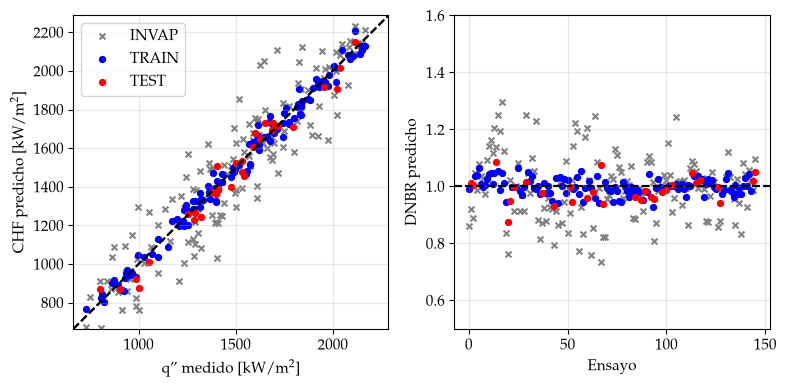
\includegraphics[width=0.95\textwidth]{Figures/chf_mfpinn_pred_final.png}
    \caption{CHF predicho contra real y DNBR por ensayo para modelo final \mfpinn{}.}
    \label{fig:chf_mfpinn_final}
\end{figure}

\subsection{Estimación de impacto}
Para estimar el impacto de la reducción del valor del \dnbrmin{} en las PLC, se utiliza el valor obtenido en evaluación de la \mfpinn{} para calcular el $\mathrm{DNBR}_\mathrm{lim}$. Luego se calcula con COBRA3-CP el valor de PLC por DNB, con los perfiles de potencia de diseño termohidráulico del IFS.
Es importante notar que esta estimación es de primer orden, puesto que el valor final del $\mathrm{DNBR}_\mathrm{lim}$ depende del límite de diseño seguro (SDL). Este límite varía por la metodología de predicción de CHF y su dependencia ante variaciones en las condiciones operativas. A priori, una predicción más robusta de CHF debería permitir reducir el $\Delta \mathrm{DNBR}_\mathrm{SDL}$, pero esa evaluación se encuentra por fuera del alcance de este trabajo ya que implica realizar todos los cálculos del diseño termohidráulico de la \cna{}.

\begin{table}[H]
	\centering
	\caption{Potencia límite de canal [MW] por DNB para metodología actual y \mfpinn{}.}
	\begin{tabular}{c c c c c c} 
        \toprule
        \multirow{2}{*}{\textbf{Metodología}} & \multicolumn{5}{c}{\textbf{Zona Hidráulica}} \\
                    & 1         & 2         & 3         & 4         & 5         \\ \hline
        Actual      & $3\,652$  & $4\,074$  & $4\,495$  & $5\,768$  & $6\,920$  \\
        \mfpinn{}   & $3\,746$  & $4\,383$  & $4\,932$  & $5\,977$  & $7\,128$  \\
        Diferencia  & $+2.6\%$  & $+7.59\%$ & $+9.72\%$ & $+3.62\%$ & $+3.01\%$ \\
		\bottomrule
	\end{tabular}
	\label{tab:mfpinn_arqs_dnbr}
\end{table}
